% Options for packages loaded elsewhere
\PassOptionsToPackage{unicode}{hyperref}
\PassOptionsToPackage{hyphens}{url}
\PassOptionsToPackage{dvipsnames,svgnames,x11names}{xcolor}
%
\documentclass[
  letterpaper,
  DIV=11,
  numbers=noendperiod]{scrartcl}

\usepackage{amsmath,amssymb}
\usepackage{iftex}
\ifPDFTeX
  \usepackage[T1]{fontenc}
  \usepackage[utf8]{inputenc}
  \usepackage{textcomp} % provide euro and other symbols
\else % if luatex or xetex
  \usepackage{unicode-math}
  \defaultfontfeatures{Scale=MatchLowercase}
  \defaultfontfeatures[\rmfamily]{Ligatures=TeX,Scale=1}
\fi
\usepackage{lmodern}
\ifPDFTeX\else  
    % xetex/luatex font selection
\fi
% Use upquote if available, for straight quotes in verbatim environments
\IfFileExists{upquote.sty}{\usepackage{upquote}}{}
\IfFileExists{microtype.sty}{% use microtype if available
  \usepackage[]{microtype}
  \UseMicrotypeSet[protrusion]{basicmath} % disable protrusion for tt fonts
}{}
\makeatletter
\@ifundefined{KOMAClassName}{% if non-KOMA class
  \IfFileExists{parskip.sty}{%
    \usepackage{parskip}
  }{% else
    \setlength{\parindent}{0pt}
    \setlength{\parskip}{6pt plus 2pt minus 1pt}}
}{% if KOMA class
  \KOMAoptions{parskip=half}}
\makeatother
\usepackage{xcolor}
\setlength{\emergencystretch}{3em} % prevent overfull lines
\setcounter{secnumdepth}{-\maxdimen} % remove section numbering
% Make \paragraph and \subparagraph free-standing
\ifx\paragraph\undefined\else
  \let\oldparagraph\paragraph
  \renewcommand{\paragraph}[1]{\oldparagraph{#1}\mbox{}}
\fi
\ifx\subparagraph\undefined\else
  \let\oldsubparagraph\subparagraph
  \renewcommand{\subparagraph}[1]{\oldsubparagraph{#1}\mbox{}}
\fi

\usepackage{color}
\usepackage{fancyvrb}
\newcommand{\VerbBar}{|}
\newcommand{\VERB}{\Verb[commandchars=\\\{\}]}
\DefineVerbatimEnvironment{Highlighting}{Verbatim}{commandchars=\\\{\}}
% Add ',fontsize=\small' for more characters per line
\usepackage{framed}
\definecolor{shadecolor}{RGB}{241,243,245}
\newenvironment{Shaded}{\begin{snugshade}}{\end{snugshade}}
\newcommand{\AlertTok}[1]{\textcolor[rgb]{0.68,0.00,0.00}{#1}}
\newcommand{\AnnotationTok}[1]{\textcolor[rgb]{0.37,0.37,0.37}{#1}}
\newcommand{\AttributeTok}[1]{\textcolor[rgb]{0.40,0.45,0.13}{#1}}
\newcommand{\BaseNTok}[1]{\textcolor[rgb]{0.68,0.00,0.00}{#1}}
\newcommand{\BuiltInTok}[1]{\textcolor[rgb]{0.00,0.23,0.31}{#1}}
\newcommand{\CharTok}[1]{\textcolor[rgb]{0.13,0.47,0.30}{#1}}
\newcommand{\CommentTok}[1]{\textcolor[rgb]{0.37,0.37,0.37}{#1}}
\newcommand{\CommentVarTok}[1]{\textcolor[rgb]{0.37,0.37,0.37}{\textit{#1}}}
\newcommand{\ConstantTok}[1]{\textcolor[rgb]{0.56,0.35,0.01}{#1}}
\newcommand{\ControlFlowTok}[1]{\textcolor[rgb]{0.00,0.23,0.31}{#1}}
\newcommand{\DataTypeTok}[1]{\textcolor[rgb]{0.68,0.00,0.00}{#1}}
\newcommand{\DecValTok}[1]{\textcolor[rgb]{0.68,0.00,0.00}{#1}}
\newcommand{\DocumentationTok}[1]{\textcolor[rgb]{0.37,0.37,0.37}{\textit{#1}}}
\newcommand{\ErrorTok}[1]{\textcolor[rgb]{0.68,0.00,0.00}{#1}}
\newcommand{\ExtensionTok}[1]{\textcolor[rgb]{0.00,0.23,0.31}{#1}}
\newcommand{\FloatTok}[1]{\textcolor[rgb]{0.68,0.00,0.00}{#1}}
\newcommand{\FunctionTok}[1]{\textcolor[rgb]{0.28,0.35,0.67}{#1}}
\newcommand{\ImportTok}[1]{\textcolor[rgb]{0.00,0.46,0.62}{#1}}
\newcommand{\InformationTok}[1]{\textcolor[rgb]{0.37,0.37,0.37}{#1}}
\newcommand{\KeywordTok}[1]{\textcolor[rgb]{0.00,0.23,0.31}{#1}}
\newcommand{\NormalTok}[1]{\textcolor[rgb]{0.00,0.23,0.31}{#1}}
\newcommand{\OperatorTok}[1]{\textcolor[rgb]{0.37,0.37,0.37}{#1}}
\newcommand{\OtherTok}[1]{\textcolor[rgb]{0.00,0.23,0.31}{#1}}
\newcommand{\PreprocessorTok}[1]{\textcolor[rgb]{0.68,0.00,0.00}{#1}}
\newcommand{\RegionMarkerTok}[1]{\textcolor[rgb]{0.00,0.23,0.31}{#1}}
\newcommand{\SpecialCharTok}[1]{\textcolor[rgb]{0.37,0.37,0.37}{#1}}
\newcommand{\SpecialStringTok}[1]{\textcolor[rgb]{0.13,0.47,0.30}{#1}}
\newcommand{\StringTok}[1]{\textcolor[rgb]{0.13,0.47,0.30}{#1}}
\newcommand{\VariableTok}[1]{\textcolor[rgb]{0.07,0.07,0.07}{#1}}
\newcommand{\VerbatimStringTok}[1]{\textcolor[rgb]{0.13,0.47,0.30}{#1}}
\newcommand{\WarningTok}[1]{\textcolor[rgb]{0.37,0.37,0.37}{\textit{#1}}}

\providecommand{\tightlist}{%
  \setlength{\itemsep}{0pt}\setlength{\parskip}{0pt}}\usepackage{longtable,booktabs,array}
\usepackage{calc} % for calculating minipage widths
% Correct order of tables after \paragraph or \subparagraph
\usepackage{etoolbox}
\makeatletter
\patchcmd\longtable{\par}{\if@noskipsec\mbox{}\fi\par}{}{}
\makeatother
% Allow footnotes in longtable head/foot
\IfFileExists{footnotehyper.sty}{\usepackage{footnotehyper}}{\usepackage{footnote}}
\makesavenoteenv{longtable}
\usepackage{graphicx}
\makeatletter
\def\maxwidth{\ifdim\Gin@nat@width>\linewidth\linewidth\else\Gin@nat@width\fi}
\def\maxheight{\ifdim\Gin@nat@height>\textheight\textheight\else\Gin@nat@height\fi}
\makeatother
% Scale images if necessary, so that they will not overflow the page
% margins by default, and it is still possible to overwrite the defaults
% using explicit options in \includegraphics[width, height, ...]{}
\setkeys{Gin}{width=\maxwidth,height=\maxheight,keepaspectratio}
% Set default figure placement to htbp
\makeatletter
\def\fps@figure{htbp}
\makeatother
\newlength{\cslhangindent}
\setlength{\cslhangindent}{1.5em}
\newlength{\csllabelwidth}
\setlength{\csllabelwidth}{3em}
\newlength{\cslentryspacingunit} % times entry-spacing
\setlength{\cslentryspacingunit}{\parskip}
\newenvironment{CSLReferences}[2] % #1 hanging-ident, #2 entry spacing
 {% don't indent paragraphs
  \setlength{\parindent}{0pt}
  % turn on hanging indent if param 1 is 1
  \ifodd #1
  \let\oldpar\par
  \def\par{\hangindent=\cslhangindent\oldpar}
  \fi
  % set entry spacing
  \setlength{\parskip}{#2\cslentryspacingunit}
 }%
 {}
\usepackage{calc}
\newcommand{\CSLBlock}[1]{#1\hfill\break}
\newcommand{\CSLLeftMargin}[1]{\parbox[t]{\csllabelwidth}{#1}}
\newcommand{\CSLRightInline}[1]{\parbox[t]{\linewidth - \csllabelwidth}{#1}\break}
\newcommand{\CSLIndent}[1]{\hspace{\cslhangindent}#1}

\KOMAoption{captions}{tableheading}
\makeatletter
\makeatother
\makeatletter
\makeatother
\makeatletter
\@ifpackageloaded{caption}{}{\usepackage{caption}}
\AtBeginDocument{%
\ifdefined\contentsname
  \renewcommand*\contentsname{Table of contents}
\else
  \newcommand\contentsname{Table of contents}
\fi
\ifdefined\listfigurename
  \renewcommand*\listfigurename{List of Figures}
\else
  \newcommand\listfigurename{List of Figures}
\fi
\ifdefined\listtablename
  \renewcommand*\listtablename{List of Tables}
\else
  \newcommand\listtablename{List of Tables}
\fi
\ifdefined\figurename
  \renewcommand*\figurename{Figure}
\else
  \newcommand\figurename{Figure}
\fi
\ifdefined\tablename
  \renewcommand*\tablename{Table}
\else
  \newcommand\tablename{Table}
\fi
}
\@ifpackageloaded{float}{}{\usepackage{float}}
\floatstyle{ruled}
\@ifundefined{c@chapter}{\newfloat{codelisting}{h}{lop}}{\newfloat{codelisting}{h}{lop}[chapter]}
\floatname{codelisting}{Listing}
\newcommand*\listoflistings{\listof{codelisting}{List of Listings}}
\makeatother
\makeatletter
\@ifpackageloaded{caption}{}{\usepackage{caption}}
\@ifpackageloaded{subcaption}{}{\usepackage{subcaption}}
\makeatother
\makeatletter
\@ifpackageloaded{tcolorbox}{}{\usepackage[skins,breakable]{tcolorbox}}
\makeatother
\makeatletter
\@ifundefined{shadecolor}{\definecolor{shadecolor}{rgb}{.97, .97, .97}}
\makeatother
\makeatletter
\makeatother
\makeatletter
\makeatother
\ifLuaTeX
  \usepackage{selnolig}  % disable illegal ligatures
\fi
\IfFileExists{bookmark.sty}{\usepackage{bookmark}}{\usepackage{hyperref}}
\IfFileExists{xurl.sty}{\usepackage{xurl}}{} % add URL line breaks if available
\urlstyle{same} % disable monospaced font for URLs
\hypersetup{
  pdftitle={Group Project: Identification of NMD sensitive RNAs and isoforms with long-read direct RNA sequencing(DRS)},
  pdfauthor={Tobia Ochsner, Michael Cibien, Gonzalo Cardenal Antolin (GonzaloCardenalAl)},
  colorlinks=true,
  linkcolor={blue},
  filecolor={Maroon},
  citecolor={Blue},
  urlcolor={Blue},
  pdfcreator={LaTeX via pandoc}}

\title{Group Project: Identification of NMD sensitive RNAs and isoforms
with long-read direct RNA sequencing(DRS)}
\author{Tobia Ochsner, Michael Cibien, Gonzalo Cardenal Antolin
(GonzaloCardenalAl)}
\date{2024-01-11}

\begin{document}
\maketitle
\ifdefined\Shaded\renewenvironment{Shaded}{\begin{tcolorbox}[frame hidden, boxrule=0pt, sharp corners, enhanced, interior hidden, borderline west={3pt}{0pt}{shadecolor}, breakable]}{\end{tcolorbox}}\fi

\hypertarget{load-packages}{%
\subsection{Load packages}\label{load-packages}}

\begin{Shaded}
\begin{Highlighting}[]
\FunctionTok{suppressPackageStartupMessages}\NormalTok{(\{}
\FunctionTok{library}\NormalTok{(limma) }
\FunctionTok{library}\NormalTok{(ggplot2)}
\FunctionTok{library}\NormalTok{(DESeq2)}
\FunctionTok{library}\NormalTok{(tximport)}
\FunctionTok{library}\NormalTok{(tidyverse)}
\FunctionTok{library}\NormalTok{(biomaRt)}
\FunctionTok{library}\NormalTok{(pheatmap)}
\FunctionTok{library}\NormalTok{(RColorBrewer)}
\FunctionTok{library}\NormalTok{(gplots)}
\FunctionTok{library}\NormalTok{(pcaExplorer)}
\FunctionTok{library}\NormalTok{(IsoformSwitchAnalyzeR)}
\FunctionTok{library}\NormalTok{(calibrate)}
\FunctionTok{library}\NormalTok{(MASS)}
\FunctionTok{library}\NormalTok{(gridExtra)}
\NormalTok{\})}
\end{Highlighting}
\end{Shaded}

\hypertarget{introduction}{%
\section{Introduction}\label{introduction}}

\hypertarget{biological-background-nmd}{%
\subsection{Biological Background --
NMD}\label{biological-background-nmd}}

Nonsense-mediated mRNA decay (NMD) is a eukaryotic pathway that is
responsible for degradation of not only aberrant, but also some
endogeneous mRNA, that would result in physiologically active proteins.
This pathway therefore plays a pivotal role in post-transcriptional gene
regulation by eliminating mRNA transcripts that could otherwise lead to
the synthesis of truncated or malfunctioning proteins. The underlying
mechanisms by which NMD selectively targets mRNAs for degradation are
not fully elucidated, however, key proteins implicated in this process
have been identified, including UPF1, an RNA helicase; SMG1, a
phosphatidylinositol-kinase-related kinase; SMG6, an endonuclease; and
SMG5 and SMG7, which function as adaptor proteins. (Karousis et al.
2021) (Karousis and Mühlemann 2022)

Historically, it was posited that the primary role of NMD was to target
mRNAs containing premature stop codons. Recent research, however,
indicates that the scope of NMD is broader, encompassing additional
features of mRNAs. To explore these additional features, particularly in
endogenous mRNAs, researchers have employed strategies such as the
knockdown of key NMD proteins. This approach increases the intracellular
concentration of NMD-targeted mRNA isoforms, facilitating their study
through subsequent RNA sequencing (RNA-seq) experiments.

\hypertarget{gene-and-isoform-expression-analysis-from-direct-rna-sequencing-drs}{%
\subsection{Gene and isoform expression analysis from direct RNA
sequencing
(DRS)}\label{gene-and-isoform-expression-analysis-from-direct-rna-sequencing-drs}}

In conventional differential gene expression analysis short-read
sequencing is widely used. However, short-read RNA sequences have
limitations in identifying and quantifying gene transcript isoforms due
to RNA fragmentation, bias introduction in the reverse transcription
into cDNA and the subsequent amplification by PCR. DRS could act as a
potential remedy to this problem, since it sequences full-length
transcripts, while also characterizing RNA modifications, polyA tails
and not needing prior PCR amplification.(Aird et al. 2011) (Steijger et
al. 2013)

It has been shown by Josie Gleeson et al that DRS has the potential to
quantify both genes and transcript isoforms in an unbiased manner
allowing for a multitude of analyses: gene and isoform quantification;
differential gene expression analysis; differential isoform usage
analysis (DUI); discovery of novel isoforms. However, the key challenges
of long-read RNA sequencing -- namely sequencing depth -- remains and
impacts the sensitivity of isoform identification with a high
probability.(Gleeson et al. 2022)

\hypertarget{goal-of-this-study}{%
\subsection{Goal of this Study}\label{goal-of-this-study}}

We were lucky to receive DRS data from a follow up project on their
paper by Dr.~Evan Karousis. They assessed endogenous targets of NMD
using a combination of long-read and short-read sequencing and found
that the juxtaposition of short-read sequencing with long-read
sequencing enabled the identification of novel NMD-targeted mRNA
isoforms. (Karousis et al. 2021)

By comparing the results of their previous work to the results of this
study, where we use DRS, we aim to answer the question of whether DRS
alone possesses sufficient resolution to delineate the full spectrum of
NMD-targeted transcripts. Data Background The data was kindly provided
by Dr.~Evangelos Karousis, who generated the data while working as
post-doctoral researcher in the laboratory of Prof.~Dr.~Oliver
Mühlemann, at the University of Bern in 2019. Knockdown experiments on
HeLa cells were performed by RNA interference (RNAi). For this, plasmids
expressing shRNAs against SMG6 and SMG7 were transfected into the
``dKD'' cells, whereas in the ``Scr'' (control) cells plasmids targeting
nothing were transfected. polyA+ mRNA was then isolated, and direct
RNA-seq was performed using the Flowcell SQK-RNA002 from Oxford
Nanopore. The MinKNOW instrument software generated fast5 files, on
which basecalling was performed using GUPPY (VERSION?) (from Oxford
Nanopore Technologies).

\hypertarget{preprocessing}{%
\section{Preprocessing}\label{preprocessing}}

\hypertarget{quality-control-qc}{%
\subsection{Quality Control (QC)}\label{quality-control-qc}}

Data was already classified in different folders based on the Quality
Control applied with Guppy. This step was done by the lab who provided
the experimental data. Two scripts were generated to confirm the
filtering heuristics applied during the quality control. We confirmed
that the filtering criteria was filtering out reads with q-score lower
than 7. (Scripts available on the github repo under the name:
``filter.r'' \& ``checkGuppyFilter.r''). We also used Nanoplot, which
provided with a report of different sequencing quality indicators
(e.g.~mean \& median read quality, weighed histogram of read
lengths\ldots). These reports are also available in the group project
GitHub repo. Also, we had reads from samples NP07 and NP08 divided in
two folders NP07 \& NP07B, and NP08 \& NP08B. The reason for this is
because during the sequencing process this stops in between so they had
to restart the sequencing. Both subsamples were then merged during the
mapping in one fatsq file. The results provided by Nanoplot confirmed
that our samples were of optimal quality (mean read quality (q-score)
\textgreater{} 7 and coherent read length distribution, sequencing error
rates, and number of reads).

The sequencing of DRS encloses a higher difficulty. As opposed to
sequencing cDNA, mRNA contains dynamic base modifications, e.g.~the most
abundant internal modification is N6-methyladenosine (m6A) (Roundtree et
al. 2017). This increases the complexity of mRNA direct sequencing and
leads to higher error rate, as when a modified nucleotide goes through
the ONT MiniON pore, the signal will be incorrect. Therefore, if we want
to study this modifications the quality criteria should be lower.

\hypertarget{mapping-and-quantification}{%
\subsection{Mapping and
quantification}\label{mapping-and-quantification}}

To map long reads, the current gold standard is using minimap2. We ran
two mappings, one to the genome and another one to the transcriptome. In
the genomic mapping, we use
\href{https://ftp.ensembl.org/pub/release-110/fasta/homo_sapiens/dna/}{Homo\_sapiens.GRCh38.dna.primary\_assembly.fa}
as the reference genome for each sample. In the transcriptome mapping,
we use the cdna reference from the Ensmbl database:
\href{https://ftp.ensembl.org/pub/release-110/fasta/homo_sapiens/cdna/}{Homo\_sapiens.GRCh38.cdna.all.fa}
.

In the quantification, we quantify the genes with Feature Counts, which
provides a mode ``-L'' tailored for long reads. The annotation file was
obtained from the Ensembl database
\href{https://ftp.ensembl.org/pub/release-110/gtf/homo_sapiens/}{Homo\_sapiens.GRCh38.110.gtf}.vWith
this mode we obtain the raw counts, needed by Deseq2 for the
differential expression analysis. For the transcripts and different
isoforms quantification we used NanoCount. NanoCount is a recently
released tool specifically developed to quantify Oxford Nanopore direct
RNA sequcing (DRS) reads. (Gleeson et al. 2022)

\hypertarget{statistical-analysis}{%
\section{Statistical Analysis}\label{statistical-analysis}}

\hypertarget{transcript-coverage}{%
\subsection{Transcript Coverage}\label{transcript-coverage}}

We run a script that outputs a series of plots and statistics. The plots
allow us to assess the coverage of the reads against the theoretical
full length of their respective isoforms. For our research purpose this
is specially helpful. DRS aims to sequence full length transcripts but,
at the time of sequencing, there can be mRNA partly degradated mRNA or
reads might not be sequence to their full length. This could lead to
ambiguous alignnments where secondary alignments would hinder the
quantification.

\begin{Shaded}
\begin{Highlighting}[]
\NormalTok{Rscript BamSlam.R rna NP05}\SpecialCharTok{{-}}\NormalTok{sorted}\SpecialCharTok{{-}}\NormalTok{transcriptomic}\SpecialCharTok{{-}}\NormalTok{aln.bam NP05\_BamSlam\_output}
\NormalTok{Rscript BamSlam.R rna NP06}\SpecialCharTok{{-}}\NormalTok{sorted}\SpecialCharTok{{-}}\NormalTok{transcriptomic}\SpecialCharTok{{-}}\NormalTok{aln.bam NP06\_BamSlam\_output}
\NormalTok{Rscript BamSlam.R rna NP07}\SpecialCharTok{{-}}\NormalTok{sorted}\SpecialCharTok{{-}}\NormalTok{transcriptomic}\SpecialCharTok{{-}}\NormalTok{aln.bam NP07\_BamSlam\_output}
\NormalTok{Rscript BamSlam.R rna NP08}\SpecialCharTok{{-}}\NormalTok{sorted}\SpecialCharTok{{-}}\NormalTok{transcriptomic}\SpecialCharTok{{-}}\NormalTok{aln.bam NP08\_BamSlam\_output}
\end{Highlighting}
\end{Shaded}

With that we can observe

(write something like this after observing results) In total, 53\% of
sequin reads were full-length compared to 38\% of 5Y reads (Figure 1F).
In comparison, using the primary alignments from minimap2 without
NanoCount filtering gave a median 5Y coverage of 0.74, with 46\% of
sequin reads and 29\% of 5Y reads being full-length. However, while a
significant proportion of reads are full-length, there is considerable
room for improvement through sequencing software advances and by
preventing degradation during RNA extraction and library preparation.

\hypertarget{import-data}{%
\subsection{Import Data}\label{import-data}}

\begin{Shaded}
\begin{Highlighting}[]
\NormalTok{samples }\OtherTok{\textless{}{-}} \FunctionTok{list.files}\NormalTok{(}\StringTok{"counts\_files"}\NormalTok{)}

\CommentTok{\#Genomic data}
\NormalTok{raw\_genomic }\OtherTok{\textless{}{-}} \FunctionTok{sapply}\NormalTok{(samples, }\ControlFlowTok{function}\NormalTok{(sample) \{}
\NormalTok{  file }\OtherTok{\textless{}{-}} \FunctionTok{paste0}\NormalTok{(}\StringTok{"counts\_files/"}\NormalTok{, sample, }\StringTok{"/"}\NormalTok{,}\StringTok{"primary{-}genomic{-}quant"}\NormalTok{)}
\NormalTok{  quant }\OtherTok{\textless{}{-}} \FunctionTok{read.table}\NormalTok{(file, }\AttributeTok{header=}\ConstantTok{TRUE}\NormalTok{, }\AttributeTok{row.names=}\DecValTok{1}\NormalTok{, }\AttributeTok{sep=}\StringTok{"}\SpecialCharTok{\textbackslash{}t}\StringTok{"}\NormalTok{)}
\NormalTok{  gene\_id }\OtherTok{\textless{}{-}} \FunctionTok{rownames}\NormalTok{(quant)}
\NormalTok{  raw }\OtherTok{\textless{}{-}}\NormalTok{ quant[,}\DecValTok{6}\NormalTok{]}
\NormalTok{  raw\_counts }\OtherTok{\textless{}{-}} \FunctionTok{setNames}\NormalTok{(raw, gene\_id)}
  \FunctionTok{return}\NormalTok{(raw\_counts)}
\NormalTok{\})}

\NormalTok{raw\_genomic }\OtherTok{\textless{}{-}} \FunctionTok{as.data.frame}\NormalTok{(raw\_genomic)}

\NormalTok{raw\_genomic }\OtherTok{\textless{}{-}}\NormalTok{ raw\_genomic }\SpecialCharTok{\%\textgreater{}\%}
  \FunctionTok{rownames\_to\_column}\NormalTok{(}\AttributeTok{var =} \StringTok{"gene\_name"}\NormalTok{) }\SpecialCharTok{\%\textgreater{}\%}
  \FunctionTok{arrange}\NormalTok{(gene\_name) }\SpecialCharTok{\%\textgreater{}\%}
  \FunctionTok{column\_to\_rownames}\NormalTok{(}\AttributeTok{var =} \StringTok{"gene\_name"}\NormalTok{)}

\FunctionTok{head}\NormalTok{(raw\_genomic)}
\end{Highlighting}
\end{Shaded}

\begin{verbatim}
                NP05-Scr1 NP06-dKD1 NP07-dKD2 NP08-Scr2
ENSG00000000003        62        50        83       100
ENSG00000000005         0         0         0         0
ENSG00000000419       118       111       184       182
ENSG00000000457         0         0         4         2
ENSG00000000460         0         0         0         0
ENSG00000000938         0         1         0         0
\end{verbatim}

\begin{Shaded}
\begin{Highlighting}[]
\CommentTok{\#Transcriptomic data}
\NormalTok{np05\_tcrm }\OtherTok{=} \FunctionTok{read.table}\NormalTok{(}\AttributeTok{file =} \StringTok{\textquotesingle{}counts\_files/NP05{-}Scr1/transcriptomic{-}quant.tsv\textquotesingle{}}\NormalTok{, }\AttributeTok{sep =} \StringTok{\textquotesingle{}}\SpecialCharTok{\textbackslash{}t}\StringTok{\textquotesingle{}}\NormalTok{, }\AttributeTok{header =} \ConstantTok{TRUE}\NormalTok{)}
\FunctionTok{head}\NormalTok{(np05\_tcrm)}
\end{Highlighting}
\end{Shaded}

\begin{verbatim}
     transcript_name         raw est_count      tpm transcript_length
1  ENST00000532829.5 0.008402080  7582.558 8402.080               912
2 ENST00000222247.10 0.006247496  5638.128 6247.496               634
3 ENST00000355968.10 0.005250192  4738.099 5250.192               818
4  ENST00000504562.1 0.004519781  4078.930 4519.781               505
5  ENST00000530721.5 0.004504106  4064.785 4504.106               796
6  ENST00000230050.4 0.004190554  3781.816 4190.554               503
\end{verbatim}

We are working with direct RNA Long-reads. As we can observe, NanoCounts
outputs est\_count and tpm. Tpm and estimated counts are not normalised
by transcript length as it is usually done with Illumina data. The
reason is that in DRS one read is supposed to represent a single
transcript molecule starting from the polyA tail, even if the fragment
doesn't extend to the 5' end.

Est\_count is the estimated counts obtained by multiplying the raw
abundance by the number of primary alignments, the latter is the
estimated counts obtained by multiplying the raw abundance by 1M. As we
observed above, the full-length transcript coverage was not higher than
30\% for any of the samples. Thereby, we decided to continue the
analysis with tpm.

\begin{Shaded}
\begin{Highlighting}[]
\NormalTok{np05\_tcrm }\OtherTok{=} \FunctionTok{data.frame}\NormalTok{(}\AttributeTok{transcript\_name =}\NormalTok{ np05\_tcrm}\SpecialCharTok{$}\NormalTok{transcript\_name, }\AttributeTok{tpm\_np05 =}\NormalTok{ np05\_tcrm}\SpecialCharTok{$}\NormalTok{tpm)}

\NormalTok{np06\_tcrm }\OtherTok{=} \FunctionTok{read.table}\NormalTok{(}\AttributeTok{file =} \StringTok{\textquotesingle{}counts\_files/NP06{-}dKD1/transcriptomic{-}quant.tsv\textquotesingle{}}\NormalTok{, }\AttributeTok{sep =} \StringTok{\textquotesingle{}}\SpecialCharTok{\textbackslash{}t}\StringTok{\textquotesingle{}}\NormalTok{, }\AttributeTok{header =} \ConstantTok{TRUE}\NormalTok{)}
\NormalTok{np06\_tcrm }\OtherTok{=} \FunctionTok{data.frame}\NormalTok{(}\AttributeTok{transcript\_name =}\NormalTok{ np06\_tcrm}\SpecialCharTok{$}\NormalTok{transcript\_name, }\AttributeTok{tpm\_np06 =}\NormalTok{ np06\_tcrm}\SpecialCharTok{$}\NormalTok{tpm)}

\NormalTok{np07\_tcrm }\OtherTok{=} \FunctionTok{read.table}\NormalTok{(}\AttributeTok{file =} \StringTok{\textquotesingle{}counts\_files/NP07{-}dKD2/transcriptomic{-}quant.tsv\textquotesingle{}}\NormalTok{, }\AttributeTok{sep =} \StringTok{\textquotesingle{}}\SpecialCharTok{\textbackslash{}t}\StringTok{\textquotesingle{}}\NormalTok{, }\AttributeTok{header =} \ConstantTok{TRUE}\NormalTok{)}
\NormalTok{np07\_tcrm }\OtherTok{=} \FunctionTok{data.frame}\NormalTok{(}\AttributeTok{transcript\_name =}\NormalTok{ np07\_tcrm}\SpecialCharTok{$}\NormalTok{transcript\_name, }\AttributeTok{tpm\_np07 =}\NormalTok{ np07\_tcrm}\SpecialCharTok{$}\NormalTok{tpm)}

\NormalTok{np08\_tcrm }\OtherTok{=} \FunctionTok{read.table}\NormalTok{(}\AttributeTok{file =} \StringTok{\textquotesingle{}counts\_files/NP08{-}Scr2/transcriptomic{-}quant.tsv\textquotesingle{}}\NormalTok{, }\AttributeTok{sep =} \StringTok{\textquotesingle{}}\SpecialCharTok{\textbackslash{}t}\StringTok{\textquotesingle{}}\NormalTok{, }\AttributeTok{header =} \ConstantTok{TRUE}\NormalTok{)}
\NormalTok{np08\_tcrm }\OtherTok{=} \FunctionTok{data.frame}\NormalTok{(}\AttributeTok{transcript\_name =}\NormalTok{ np08\_tcrm}\SpecialCharTok{$}\NormalTok{transcript\_name, }\AttributeTok{tpm\_np08 =}\NormalTok{ np08\_tcrm}\SpecialCharTok{$}\NormalTok{tpm)}

\NormalTok{tpm\_transcriptome }\OtherTok{\textless{}{-}} \FunctionTok{Reduce}\NormalTok{(}\ControlFlowTok{function}\NormalTok{(x, y) }\FunctionTok{merge}\NormalTok{(x, y, }\AttributeTok{by =} \StringTok{"transcript\_name"}\NormalTok{, }\AttributeTok{all =} \ConstantTok{TRUE}\NormalTok{), }\FunctionTok{list}\NormalTok{(np05\_tcrm, np06\_tcrm, np07\_tcrm, np08\_tcrm))}

\CommentTok{\# Rename columns to specify the dataset source}
\NormalTok{tpm\_transcriptome }\OtherTok{\textless{}{-}} \FunctionTok{as.data.frame}\NormalTok{(tpm\_transcriptome)}
\NormalTok{tpm\_transcriptome  }\OtherTok{\textless{}{-}}\NormalTok{ tpm\_transcriptome  }\SpecialCharTok{\%\textgreater{}\%}
  \FunctionTok{arrange}\NormalTok{(transcript\_name) }\SpecialCharTok{\%\textgreater{}\%}
  \FunctionTok{column\_to\_rownames}\NormalTok{(}\AttributeTok{var =} \StringTok{"transcript\_name"}\NormalTok{)}

\FunctionTok{head}\NormalTok{(tpm\_transcriptome)}
\end{Highlighting}
\end{Shaded}

\begin{verbatim}
                      tpm_np05    tpm_np06   tpm_np07   tpm_np08
ENST00000000233.10 309.1542913 240.5310318 283.702478 336.004874
ENST00000000412.8   76.4575129  96.7413900  93.289284  94.624125
ENST00000000442.11   7.9517822   1.4499922   2.569157   8.118034
ENST00000001008.6    0.5540399   0.0000000   0.000000   0.000000
ENST00000001146.7    0.0000000   0.5624499   0.804218   2.201090
ENST00000002125.9   11.0807987  10.1240990   7.036907   9.337958
\end{verbatim}

\hypertarget{exploratory-analysis}{%
\subsection{Exploratory Analysis}\label{exploratory-analysis}}

Once we obtain the genomic and transcriptomic counts of our samples, we
run a initial exploratory analysis.

\begin{Shaded}
\begin{Highlighting}[]
\FunctionTok{colSums}\NormalTok{(raw\_genomic)}
\end{Highlighting}
\end{Shaded}

\begin{verbatim}
NP05-Scr1 NP06-dKD1 NP07-dKD2 NP08-Scr2 
   882803    877859   1239173   1323920 
\end{verbatim}

\begin{Shaded}
\begin{Highlighting}[]
\FunctionTok{colSums}\NormalTok{(tpm\_transcriptome)}
\end{Highlighting}
\end{Shaded}

\begin{verbatim}
tpm_np05 tpm_np06 tpm_np07 tpm_np08 
   1e+06    1e+06    1e+06    1e+06 
\end{verbatim}

The transcript counts have the same number of total counts between
samples, whereas the raw genomic counts have different number of total
counts. We can normalise between the samples with scaling factors to
have the same number of total counts between samples.

\begin{Shaded}
\begin{Highlighting}[]
\NormalTok{median\_all\_counts }\OtherTok{=} \FunctionTok{median}\NormalTok{(}\FunctionTok{colSums}\NormalTok{(raw\_genomic))}
\NormalTok{scaling\_factors }\OtherTok{=} \FunctionTok{median}\NormalTok{(}\FunctionTok{colSums}\NormalTok{(raw\_genomic))}\SpecialCharTok{/}\FunctionTok{colSums}\NormalTok{(raw\_genomic)}
\NormalTok{normalised\_genomic}\OtherTok{=}\FunctionTok{sweep}\NormalTok{(raw\_genomic, }\DecValTok{2}\NormalTok{, scaling\_factors, }\StringTok{\textasciigrave{}}\AttributeTok{*}\StringTok{\textasciigrave{}}\NormalTok{)}

\FunctionTok{colSums}\NormalTok{(normalised\_genomic)}
\end{Highlighting}
\end{Shaded}

\begin{verbatim}
NP05-Scr1 NP06-dKD1 NP07-dKD2 NP08-Scr2 
  1060988   1060988   1060988   1060988 
\end{verbatim}

\begin{Shaded}
\begin{Highlighting}[]
\NormalTok{log\_normalised\_genomic}\OtherTok{=}\FunctionTok{log1p}\NormalTok{(normalised\_genomic)}

\NormalTok{melted\_data }\OtherTok{\textless{}{-}}\NormalTok{ reshape2}\SpecialCharTok{::}\FunctionTok{melt}\NormalTok{(log\_normalised\_genomic)}
\end{Highlighting}
\end{Shaded}

\begin{verbatim}
No id variables; using all as measure variables
\end{verbatim}

\begin{Shaded}
\begin{Highlighting}[]
\FunctionTok{colnames}\NormalTok{(melted\_data) }\OtherTok{\textless{}{-}} \FunctionTok{c}\NormalTok{(}\StringTok{"sample"}\NormalTok{,}\StringTok{"Log\_normalised\_expression"}\NormalTok{)}

\NormalTok{violin\_plot\_allgenes }\OtherTok{\textless{}{-}} \FunctionTok{ggplot}\NormalTok{(melted\_data, }\FunctionTok{aes}\NormalTok{(}\AttributeTok{x=}\NormalTok{sample, }\AttributeTok{y=}\NormalTok{Log\_normalised\_expression, }\AttributeTok{fill=}\NormalTok{sample)) }\SpecialCharTok{+}
  \FunctionTok{geom\_violin}\NormalTok{() }\SpecialCharTok{+}
  \FunctionTok{labs}\NormalTok{(}\AttributeTok{title=}\StringTok{\textquotesingle{}Violoin Plot of all samples Gene Log Expression Distribution\textquotesingle{}}\NormalTok{, }\AttributeTok{x=}\StringTok{\textquotesingle{}samples\textquotesingle{}}\NormalTok{,}\AttributeTok{y=}\StringTok{\textquotesingle{}Log expression\textquotesingle{}}\NormalTok{)}
  \FunctionTok{theme}\NormalTok{(}\AttributeTok{plot.title =} \FunctionTok{element\_text}\NormalTok{(}\AttributeTok{hjust =} \FloatTok{0.5}\NormalTok{))}
\end{Highlighting}
\end{Shaded}

\begin{verbatim}
List of 1
 $ plot.title:List of 11
  ..$ family       : NULL
  ..$ face         : NULL
  ..$ colour       : NULL
  ..$ size         : NULL
  ..$ hjust        : num 0.5
  ..$ vjust        : NULL
  ..$ angle        : NULL
  ..$ lineheight   : NULL
  ..$ margin       : NULL
  ..$ debug        : NULL
  ..$ inherit.blank: logi FALSE
  ..- attr(*, "class")= chr [1:2] "element_text" "element"
 - attr(*, "class")= chr [1:2] "theme" "gg"
 - attr(*, "complete")= logi FALSE
 - attr(*, "validate")= logi TRUE
\end{verbatim}

\begin{Shaded}
\begin{Highlighting}[]
\FunctionTok{print}\NormalTok{(violin\_plot\_allgenes)}
\end{Highlighting}
\end{Shaded}

\begin{figure}[H]

{\centering 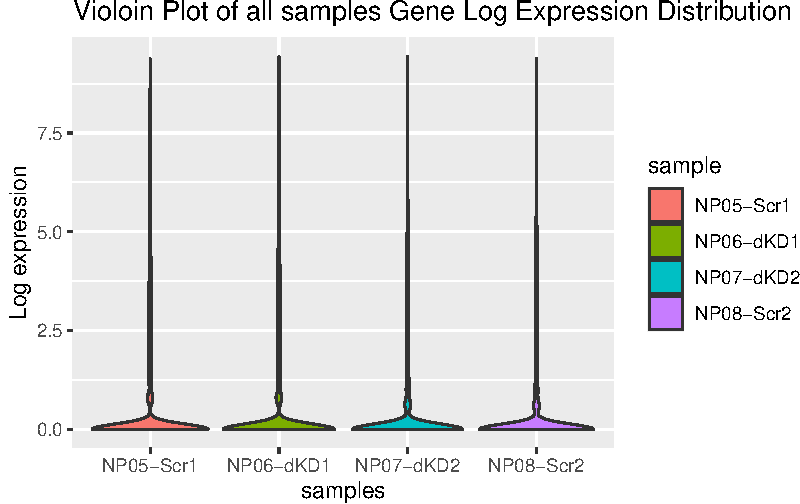
\includegraphics{intro-STAT-GroupProject_files/figure-pdf/unnamed-chunk-6-1.pdf}

}

\end{figure}

All samples have similar gene expression distributions by looking at the
violin plots.

\begin{Shaded}
\begin{Highlighting}[]
\NormalTok{avg\_genomic }\OtherTok{\textless{}{-}} \FunctionTok{rowMeans}\NormalTok{(raw\_genomic)}

\FunctionTok{par}\NormalTok{(}\AttributeTok{mfrow =} \FunctionTok{c}\NormalTok{(}\DecValTok{1}\NormalTok{, }\DecValTok{2}\NormalTok{))}
\FunctionTok{layout}\NormalTok{(}\FunctionTok{matrix}\NormalTok{(}\DecValTok{1}\SpecialCharTok{:}\DecValTok{2}\NormalTok{, }\AttributeTok{nrow =} \DecValTok{1}\NormalTok{))}
\FunctionTok{par}\NormalTok{(}\AttributeTok{mar =} \FunctionTok{c}\NormalTok{(}\DecValTok{3}\NormalTok{, }\DecValTok{3}\NormalTok{, }\DecValTok{2}\NormalTok{, }\DecValTok{1}\NormalTok{)) }
\FunctionTok{hist}\NormalTok{(avg\_genomic)}
\FunctionTok{hist}\NormalTok{(}\FunctionTok{log1p}\NormalTok{(avg\_genomic))}

\NormalTok{layout }\OtherTok{\textless{}{-}} \FunctionTok{matrix}\NormalTok{(}\FunctionTok{c}\NormalTok{(}\DecValTok{1}\NormalTok{, }\DecValTok{2}\NormalTok{), }\AttributeTok{nrow =} \DecValTok{1}\NormalTok{)}

\NormalTok{plot }\OtherTok{\textless{}{-}} \FunctionTok{ggplot}\NormalTok{(}\AttributeTok{data =} \FunctionTok{as.data.frame}\NormalTok{(avg\_genomic), }\AttributeTok{mapping =} \FunctionTok{aes}\NormalTok{(}\AttributeTok{x =}\NormalTok{ avg\_genomic)) }\SpecialCharTok{+}
  \FunctionTok{geom\_histogram}\NormalTok{(}
    \AttributeTok{color =} \StringTok{"white"}\NormalTok{,}
    \AttributeTok{fill =} \FunctionTok{brewer.pal}\NormalTok{(}\AttributeTok{n =} \DecValTok{3}\NormalTok{, }\AttributeTok{name =} \StringTok{"Set1"}\NormalTok{)[}\DecValTok{2}\NormalTok{],}
    \AttributeTok{bins =} \DecValTok{50}
\NormalTok{  ) }\SpecialCharTok{+}
  \FunctionTok{labs}\NormalTok{(}\AttributeTok{title =} \StringTok{"Distribution of average expression values of all genes"}\NormalTok{,}
       \AttributeTok{x =} \StringTok{"Average expression"}\NormalTok{,}
       \AttributeTok{y =} \StringTok{"Count"}\NormalTok{) }\SpecialCharTok{+}
  \FunctionTok{theme\_minimal}\NormalTok{() }\SpecialCharTok{+}
  \FunctionTok{theme}\NormalTok{(}\AttributeTok{plot.title =} \FunctionTok{element\_text}\NormalTok{(}\AttributeTok{hjust =} \FloatTok{0.5}\NormalTok{))}

\NormalTok{log\_plot }\OtherTok{\textless{}{-}} \FunctionTok{ggplot}\NormalTok{(}\AttributeTok{data =} \FunctionTok{as.data.frame}\NormalTok{(avg\_genomic), }\AttributeTok{mapping =} \FunctionTok{aes}\NormalTok{(}\AttributeTok{x =} \FunctionTok{log}\NormalTok{(avg\_genomic }\SpecialCharTok{+} \DecValTok{1}\NormalTok{))) }\SpecialCharTok{+}
  \FunctionTok{geom\_histogram}\NormalTok{(}
    \AttributeTok{color =} \StringTok{"white"}\NormalTok{,}
    \AttributeTok{fill =} \FunctionTok{brewer.pal}\NormalTok{(}\AttributeTok{n =} \DecValTok{3}\NormalTok{, }\AttributeTok{name =} \StringTok{"Set1"}\NormalTok{)[}\DecValTok{2}\NormalTok{],}
    \AttributeTok{bins =} \DecValTok{50}
\NormalTok{  ) }\SpecialCharTok{+}
  \FunctionTok{labs}\NormalTok{(}\AttributeTok{title =} \StringTok{"Log Distribution of average expression values of all genes"}\NormalTok{,}
       \AttributeTok{x =} \StringTok{"log10(Average expression + 1)"}\NormalTok{,}
       \AttributeTok{y =} \StringTok{"Count"}\NormalTok{) }\SpecialCharTok{+}
  \FunctionTok{theme\_minimal}\NormalTok{() }\SpecialCharTok{+}
  \FunctionTok{theme}\NormalTok{(}\AttributeTok{plot.title =} \FunctionTok{element\_text}\NormalTok{(}\AttributeTok{hjust =} \FloatTok{0.5}\NormalTok{))}

\CommentTok{\# Arrange and display the plots}
\FunctionTok{grid.arrange}\NormalTok{(plot, log\_plot, }\AttributeTok{layout\_matrix =}\NormalTok{ layout)}
\end{Highlighting}
\end{Shaded}

\begin{Shaded}
\begin{Highlighting}[]
\NormalTok{avg\_genomic }\OtherTok{\textless{}{-}} \FunctionTok{rowMeans}\NormalTok{(raw\_genomic)}
\NormalTok{layout }\OtherTok{\textless{}{-}} \FunctionTok{matrix}\NormalTok{(}\FunctionTok{c}\NormalTok{(}\DecValTok{1}\NormalTok{, }\DecValTok{2}\NormalTok{, }\DecValTok{3}\NormalTok{, }\DecValTok{4}\NormalTok{), }\AttributeTok{nrow =} \DecValTok{2}\NormalTok{, }\AttributeTok{byrow =} \ConstantTok{TRUE}\NormalTok{)}

\NormalTok{plot\_1 }\OtherTok{\textless{}{-}} \FunctionTok{ggplot}\NormalTok{(}\AttributeTok{data =} \FunctionTok{as.data.frame}\NormalTok{(avg\_genomic), }\AttributeTok{mapping =}  \FunctionTok{aes}\NormalTok{(}\AttributeTok{x =}\NormalTok{ avg\_genomic)) }\SpecialCharTok{+}
  \FunctionTok{geom\_histogram}\NormalTok{(}
    \AttributeTok{color =} \StringTok{"white"}\NormalTok{,}
    \AttributeTok{fill =} \FunctionTok{brewer.pal}\NormalTok{(}\AttributeTok{n =} \DecValTok{3}\NormalTok{, }\AttributeTok{name =} \StringTok{"Set1"}\NormalTok{)[}\DecValTok{2}\NormalTok{],}
    \AttributeTok{bins =} \DecValTok{50}
\NormalTok{  ) }\SpecialCharTok{+}
  \FunctionTok{scale\_x\_continuous}\NormalTok{(}
    \AttributeTok{breaks =} \FunctionTok{c}\NormalTok{(}\DecValTok{0}\NormalTok{, }\DecValTok{1}\NormalTok{, }\DecValTok{10}\NormalTok{, }\DecValTok{100}\NormalTok{, }\DecValTok{1000}\NormalTok{, }\DecValTok{10000}\NormalTok{, }\DecValTok{20000}\NormalTok{),}
    \AttributeTok{trans =} \StringTok{"log1p"}\NormalTok{,}
    \AttributeTok{expand =} \FunctionTok{c}\NormalTok{(}\DecValTok{0}\NormalTok{, }\DecValTok{0}\NormalTok{)}
\NormalTok{  ) }\SpecialCharTok{+}
  \FunctionTok{scale\_y\_continuous}\NormalTok{(}\AttributeTok{breaks =} \FunctionTok{c}\NormalTok{(}\DecValTok{0}\NormalTok{, }\DecValTok{1}\NormalTok{),}
                     \AttributeTok{expand =} \FunctionTok{c}\NormalTok{(}\DecValTok{0}\NormalTok{, }\DecValTok{0}\NormalTok{),}
                     \AttributeTok{trans =} \StringTok{"log1p"}\NormalTok{) }\SpecialCharTok{+}
  \FunctionTok{labs}\NormalTok{(}\AttributeTok{title =} \StringTok{"Distribution of average expression values of all genes"}\NormalTok{,}
       \AttributeTok{x =} \StringTok{"log1p(Average expression)"}\NormalTok{,}
       \AttributeTok{y =} \StringTok{"log1p(Count)"}\NormalTok{) }\SpecialCharTok{+}
  \FunctionTok{theme\_minimal}\NormalTok{() }\SpecialCharTok{+}
  \FunctionTok{theme}\NormalTok{(}\AttributeTok{plot.title =} \FunctionTok{element\_text}\NormalTok{(}\AttributeTok{hjust =} \FloatTok{0.5}\NormalTok{, }\AttributeTok{size =} \DecValTok{5}\NormalTok{))}

\NormalTok{num\_detected\_genes }\OtherTok{\textless{}{-}} \FunctionTok{rowSums}\NormalTok{(raw\_genomic }\SpecialCharTok{\textgreater{}} \DecValTok{0}\NormalTok{)}

\NormalTok{plot\_2 }\OtherTok{\textless{}{-}} \FunctionTok{ggplot}\NormalTok{(}\AttributeTok{data =} \FunctionTok{as.data.frame}\NormalTok{(num\_detected\_genes), }\AttributeTok{mapping =}  \FunctionTok{aes}\NormalTok{(}\AttributeTok{x =}\NormalTok{ num\_detected\_genes)) }\SpecialCharTok{+}
  \FunctionTok{geom\_histogram}\NormalTok{(}
    \AttributeTok{color =} \StringTok{"white"}\NormalTok{,}
    \AttributeTok{fill =} \FunctionTok{brewer.pal}\NormalTok{(}\AttributeTok{n =} \DecValTok{3}\NormalTok{, }\AttributeTok{name =} \StringTok{"Set1"}\NormalTok{)[}\DecValTok{2}\NormalTok{],}
    \AttributeTok{bins =} \DecValTok{23}
\NormalTok{  ) }\SpecialCharTok{+}
  \FunctionTok{labs}\NormalTok{(}\AttributeTok{title =} \StringTok{"Distribution of number samples in which each gene is detected"}\NormalTok{,}
       \AttributeTok{x =} \StringTok{"Number of samples"}\NormalTok{,}
       \AttributeTok{y =} \StringTok{"Count"}\NormalTok{) }\SpecialCharTok{+}
  \FunctionTok{theme\_minimal}\NormalTok{() }\SpecialCharTok{+}
  \FunctionTok{theme}\NormalTok{(}\AttributeTok{plot.title =} \FunctionTok{element\_text}\NormalTok{(}\AttributeTok{hjust =} \FloatTok{0.5}\NormalTok{, }\AttributeTok{size =} \DecValTok{5}\NormalTok{))}


\CommentTok{\# filter expressed genes }
\CommentTok{\# threshold: genes must be detected in at least half of the samples}
\CommentTok{\#            or the average counts must be \textgreater{}= 1}

\NormalTok{expressed }\OtherTok{\textless{}{-}} \FunctionTok{rowSums}\NormalTok{(raw\_genomic) }\SpecialCharTok{\textgreater{}=} \DecValTok{5}
\NormalTok{num\_filtered\_expressed\_genes }\OtherTok{\textless{}{-}} \FunctionTok{rowSums}\NormalTok{(raw\_genomic[expressed,] }\SpecialCharTok{\textgreater{}} \DecValTok{0}\NormalTok{)}

\NormalTok{avg\_genomic }\OtherTok{\textless{}{-}} \FunctionTok{data.frame}\NormalTok{(avg\_genomic)}
\NormalTok{plot\_3 }\OtherTok{\textless{}{-}} \FunctionTok{ggplot}\NormalTok{(}\AttributeTok{data =} \FunctionTok{as.data.frame}\NormalTok{(avg\_genomic[expressed,]), }\AttributeTok{mapping =}  \FunctionTok{aes}\NormalTok{(}\AttributeTok{x =}\NormalTok{ avg\_genomic[expressed,])) }\SpecialCharTok{+}
  \FunctionTok{geom\_histogram}\NormalTok{(}
    \AttributeTok{color =} \StringTok{"white"}\NormalTok{,}
    \AttributeTok{fill =} \FunctionTok{brewer.pal}\NormalTok{(}\AttributeTok{n =} \DecValTok{3}\NormalTok{, }\AttributeTok{name =} \StringTok{"Set1"}\NormalTok{)[}\DecValTok{2}\NormalTok{],}
    \AttributeTok{bins =} \DecValTok{50}
\NormalTok{  ) }\SpecialCharTok{+}
  \FunctionTok{scale\_x\_continuous}\NormalTok{(}
    \AttributeTok{breaks =} \FunctionTok{c}\NormalTok{(}\DecValTok{0}\NormalTok{, }\DecValTok{1}\NormalTok{, }\DecValTok{10}\NormalTok{, }\DecValTok{100}\NormalTok{, }\DecValTok{1000}\NormalTok{, }\DecValTok{10000}\NormalTok{, }\DecValTok{20000}\NormalTok{),}
    \AttributeTok{trans =} \StringTok{"log1p"}\NormalTok{,}
    \AttributeTok{expand =} \FunctionTok{c}\NormalTok{(}\DecValTok{0}\NormalTok{, }\DecValTok{0}\NormalTok{)}
\NormalTok{  ) }\SpecialCharTok{+}
  \FunctionTok{scale\_y\_continuous}\NormalTok{(}\AttributeTok{breaks =} \FunctionTok{c}\NormalTok{(}\DecValTok{0}\NormalTok{, }\DecValTok{1}\NormalTok{),}
                     \AttributeTok{expand =} \FunctionTok{c}\NormalTok{(}\DecValTok{0}\NormalTok{, }\DecValTok{0}\NormalTok{),}
                     \AttributeTok{trans =} \StringTok{"log1p"}\NormalTok{) }\SpecialCharTok{+}
  \FunctionTok{labs}\NormalTok{(}\AttributeTok{title =} \StringTok{"Distribution of average expression values of all genes after filtering"}\NormalTok{,}
       \AttributeTok{x =} \StringTok{"log1p(Average expression)"}\NormalTok{,}
       \AttributeTok{y =} \StringTok{"log1p(Count)"}\NormalTok{) }\SpecialCharTok{+}
  \FunctionTok{theme\_minimal}\NormalTok{() }\SpecialCharTok{+}
  \FunctionTok{theme}\NormalTok{(}\AttributeTok{plot.title =} \FunctionTok{element\_text}\NormalTok{(}\AttributeTok{hjust =} \FloatTok{0.5}\NormalTok{,  }\AttributeTok{size =} \DecValTok{5}\NormalTok{))}

\NormalTok{plot\_4 }\OtherTok{\textless{}{-}} \FunctionTok{ggplot}\NormalTok{(}\AttributeTok{data =} \FunctionTok{as.data.frame}\NormalTok{(num\_filtered\_expressed\_genes), }\AttributeTok{mapping =}  \FunctionTok{aes}\NormalTok{(}\AttributeTok{x =}\NormalTok{ num\_filtered\_expressed\_genes)) }\SpecialCharTok{+}
  \FunctionTok{geom\_histogram}\NormalTok{(}
    \AttributeTok{color =} \StringTok{"white"}\NormalTok{,}
    \AttributeTok{fill =} \FunctionTok{brewer.pal}\NormalTok{(}\AttributeTok{n =} \DecValTok{3}\NormalTok{, }\AttributeTok{name =} \StringTok{"Set1"}\NormalTok{)[}\DecValTok{2}\NormalTok{],}
    \AttributeTok{bins =} \DecValTok{23}
\NormalTok{  ) }\SpecialCharTok{+}
  \FunctionTok{labs}\NormalTok{(}\AttributeTok{title =} \StringTok{"Distribution of number samples in which each gene is detected after filtering"}\NormalTok{,}
       \AttributeTok{x =} \StringTok{"Number of samples"}\NormalTok{,}
       \AttributeTok{y =} \StringTok{"Count"}\NormalTok{) }\SpecialCharTok{+}
  \FunctionTok{theme\_minimal}\NormalTok{() }\SpecialCharTok{+}
  \FunctionTok{theme}\NormalTok{(}\AttributeTok{plot.title =} \FunctionTok{element\_text}\NormalTok{(}\AttributeTok{hjust =} \FloatTok{0.5}\NormalTok{,  }\AttributeTok{size =} \DecValTok{5}\NormalTok{))}

\FunctionTok{grid.arrange}\NormalTok{(plot\_1, plot\_2, plot\_3, plot\_4, }\AttributeTok{layout\_matrix =}\NormalTok{ layout)}
\end{Highlighting}
\end{Shaded}

\begin{figure}[H]

{\centering 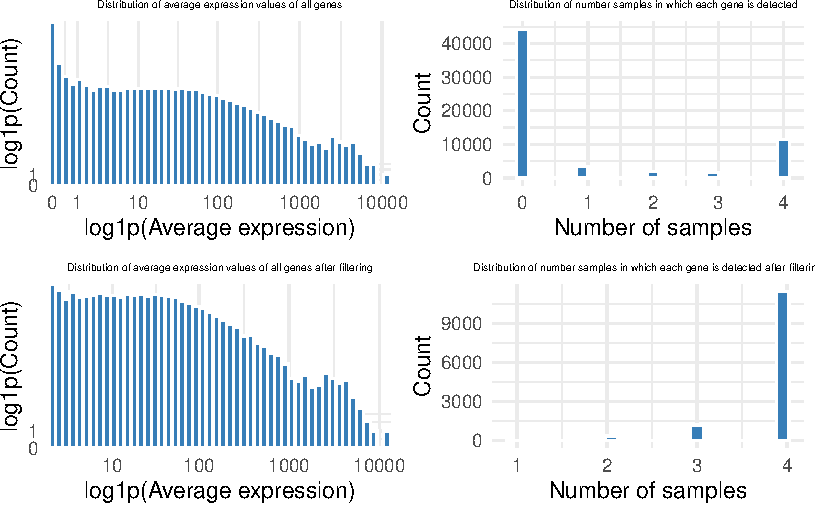
\includegraphics{intro-STAT-GroupProject_files/figure-pdf/unnamed-chunk-8-1.pdf}

}

\end{figure}

We filter our genes to remove very low counts, removing genes with
counts \textless{} 5. By looking at the plots in the right size of the
figure, we can observe that our filtering criteria filtered not only all
the genes not expressed in any of the samples but also most of the genes
only expressed in one individual sample.

\begin{Shaded}
\begin{Highlighting}[]
\CommentTok{\#Plot heatmap}
\NormalTok{corr\_pearson }\OtherTok{\textless{}{-}} \FunctionTok{cor}\NormalTok{(}\FunctionTok{log1p}\NormalTok{(raw\_genomic[expressed,]), }\AttributeTok{method =} \StringTok{"spearman"}\NormalTok{)}
\FunctionTok{pheatmap}\NormalTok{(corr\_pearson)}
\end{Highlighting}
\end{Shaded}

\begin{figure}[H]

{\centering 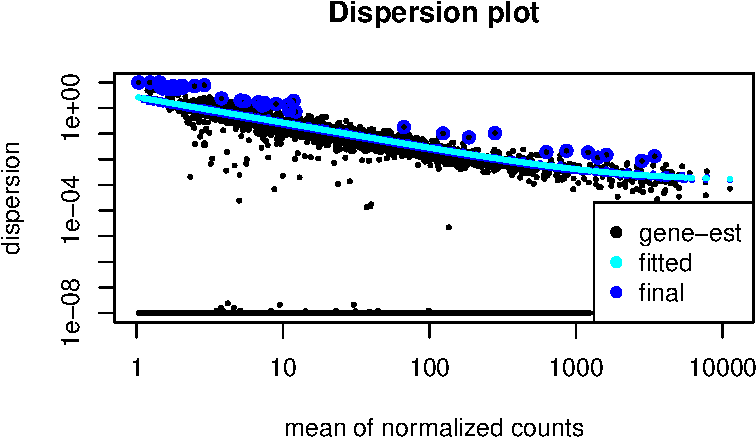
\includegraphics{intro-STAT-GroupProject_files/figure-pdf/unnamed-chunk-9-1.pdf}

}

\end{figure}

The control and the knockdown samples correlate, which indicates there
is a differential expression between the knockdown and the control. This
again indicates the NMD knockdown might be working and causing a
differential gene expression.

\hypertarget{differential-gene-expression-analysis}{%
\subsection{Differential Gene Expression
Analysis}\label{differential-gene-expression-analysis}}

\begin{Shaded}
\begin{Highlighting}[]
\CommentTok{\#DESeq input}
\NormalTok{raw\_genomic}\OtherTok{\textless{}{-}} \FunctionTok{as.matrix}\NormalTok{(raw\_genomic[expressed,])}
\NormalTok{condition }\OtherTok{\textless{}{-}} \FunctionTok{factor}\NormalTok{(}\FunctionTok{c}\NormalTok{(}\StringTok{"control"}\NormalTok{,}\StringTok{"knockdown"}\NormalTok{,}\StringTok{"knockdown"}\NormalTok{,}\StringTok{"control"}\NormalTok{)) }\CommentTok{\#NP05{-}Scr1, NP06{-}dKD1, NP07{-}dKD2, NP08{-}Scr2}
\NormalTok{(coldata }\OtherTok{\textless{}{-}} \FunctionTok{data.frame}\NormalTok{(}\AttributeTok{row.names=}\FunctionTok{colnames}\NormalTok{(raw\_genomic), condition))}
\end{Highlighting}
\end{Shaded}

\begin{verbatim}
          condition
NP05-Scr1   control
NP06-dKD1 knockdown
NP07-dKD2 knockdown
NP08-Scr2   control
\end{verbatim}

\begin{Shaded}
\begin{Highlighting}[]
\CommentTok{\# Make DESeq dataset}
\NormalTok{dds }\OtherTok{\textless{}{-}} \FunctionTok{DESeqDataSetFromMatrix}\NormalTok{(}\AttributeTok{countData=}\NormalTok{raw\_genomic, }\AttributeTok{colData=}\NormalTok{coldata, }\AttributeTok{design=}\SpecialCharTok{\textasciitilde{}}\NormalTok{condition)}
\NormalTok{dds}
\end{Highlighting}
\end{Shaded}

\begin{verbatim}
class: DESeqDataSet 
dim: 12939 4 
metadata(1): version
assays(1): counts
rownames(12939): ENSG00000000003 ENSG00000000419 ... ENSG00000292366
  ENSG00000292372
rowData names(0):
colnames(4): NP05-Scr1 NP06-dKD1 NP07-dKD2 NP08-Scr2
colData names(1): condition
\end{verbatim}

\begin{Shaded}
\begin{Highlighting}[]
\CommentTok{\# Run DESeq2 pipeline}
\NormalTok{dds }\OtherTok{\textless{}{-}} \FunctionTok{DESeq}\NormalTok{(dds)}
\NormalTok{res }\OtherTok{\textless{}{-}}\NormalTok{ DESeq2}\SpecialCharTok{::}\FunctionTok{results}\NormalTok{(dds)}
\NormalTok{res}
\end{Highlighting}
\end{Shaded}

\begin{verbatim}
log2 fold change (MLE): condition knockdown vs control 
Wald test p-value: condition knockdown vs control 
DataFrame with 12939 rows and 6 columns
                 baseMean log2FoldChange     lfcSE       stat    pvalue
                <numeric>      <numeric> <numeric>  <numeric> <numeric>
ENSG00000000003  71.15309     -0.3257766  0.316642 -1.0288486  0.303551
ENSG00000000419 143.64052     -0.0706369  0.227744 -0.3101595  0.756440
ENSG00000000457   1.24498      0.9671047  2.550072  0.3792461  0.704505
ENSG00000001036  16.90446      0.0497611  0.664812  0.0748498  0.940334
ENSG00000001084   7.01765     -0.5919908  0.995149 -0.5948766  0.551926
...                   ...            ...       ...        ...       ...
ENSG00000292348 189.15052      0.1779944  0.197726   0.900206 0.3680104
ENSG00000292357  10.22278      1.4422616  0.848663   1.699451 0.0892342
ENSG00000292358  41.25677     -0.0652091  0.411644  -0.158411 0.8741326
ENSG00000292366  31.81156      0.7044188  0.484724   1.453238 0.1461577
ENSG00000292372   3.62745      1.2337631  1.475494   0.836170 0.4030594
                     padj
                <numeric>
ENSG00000000003  0.562073
ENSG00000000419  0.890040
ENSG00000000457        NA
ENSG00000001036  0.977413
ENSG00000001084  0.764897
...                   ...
ENSG00000292348  0.624072
ENSG00000292357  0.264707
ENSG00000292358  0.949564
ENSG00000292366  0.363055
ENSG00000292372        NA
\end{verbatim}

\begin{Shaded}
\begin{Highlighting}[]
\CommentTok{\#DESeq2 results}
\FunctionTok{table}\NormalTok{(res}\SpecialCharTok{$}\NormalTok{padj}\SpecialCharTok{\textless{}}\FloatTok{0.05}\NormalTok{)}
\end{Highlighting}
\end{Shaded}

\begin{verbatim}

FALSE  TRUE 
 7271  1654 
\end{verbatim}

\begin{Shaded}
\begin{Highlighting}[]
\NormalTok{res }\OtherTok{\textless{}{-}}\NormalTok{ res[}\FunctionTok{order}\NormalTok{(res}\SpecialCharTok{$}\NormalTok{padj), ]}

\CommentTok{\# Merge with normalized count data}
\NormalTok{resdata }\OtherTok{\textless{}{-}} \FunctionTok{merge}\NormalTok{(}\FunctionTok{as.data.frame}\NormalTok{(res), }\FunctionTok{as.data.frame}\NormalTok{(}\FunctionTok{counts}\NormalTok{(dds, }\AttributeTok{normalized=}\ConstantTok{TRUE}\NormalTok{)), }\AttributeTok{by=}\StringTok{"row.names"}\NormalTok{, }\AttributeTok{sort=}\ConstantTok{FALSE}\NormalTok{)}
\FunctionTok{names}\NormalTok{(resdata)[}\DecValTok{1}\NormalTok{] }\OtherTok{\textless{}{-}} \StringTok{"Gene"}
\NormalTok{resdata}\SpecialCharTok{$}\NormalTok{DE }\OtherTok{\textless{}{-}}\NormalTok{resdata}\SpecialCharTok{$}\NormalTok{padj}\SpecialCharTok{\textless{}}\FloatTok{0.05}
\FunctionTok{head}\NormalTok{(resdata)}
\end{Highlighting}
\end{Shaded}

\begin{verbatim}
             Gene  baseMean log2FoldChange      lfcSE     stat        pvalue
1 ENSG00000224032 1000.8274       4.307767 0.13936391 30.91021 8.709885e-210
2 ENSG00000169242  886.1724       3.720117 0.13127462 28.33843 1.162292e-176
3 ENSG00000107262 1221.1706       2.555759 0.09930271 25.73705 4.501466e-146
4 ENSG00000210082 7819.4672       1.723809 0.06830571 25.23668 1.586237e-140
5 ENSG00000116761  605.5634       3.286235 0.14590196 22.52358 2.438256e-112
6 ENSG00000211459 3961.3526       1.490358 0.06967320 21.39070 1.630984e-101
           padj NP05-Scr1 NP06-dKD1 NP07-dKD2 NP08-Scr2   DE
1 7.773572e-206   89.5916  1837.283  1975.093  101.3427 TRUE
2 5.186729e-173  130.0919  1611.611  1681.869  121.1169 TRUE
3 1.339186e-142  351.0027  2086.889  2088.384  358.4071 TRUE
4 3.539291e-137 3424.1174 11737.182 12278.729 3837.8402 TRUE
5 4.352287e-109  101.8644  1114.679  1084.593  121.1169 TRUE
6  2.426088e-98 2055.6977  6056.650  5632.055 2101.0074 TRUE
\end{verbatim}

\begin{Shaded}
\begin{Highlighting}[]
\CommentTok{\# Plot dispersions}
\FunctionTok{plotDispEsts}\NormalTok{(dds, }\AttributeTok{main=}\StringTok{"Dispersion plot"}\NormalTok{, }\AttributeTok{genecol =} \StringTok{"black"}\NormalTok{, }\AttributeTok{fitcol =} \StringTok{"cyan"}\NormalTok{, }\AttributeTok{finalcol =} \StringTok{"blue"}\NormalTok{, }\AttributeTok{legend =} \ConstantTok{TRUE}\NormalTok{)}
\end{Highlighting}
\end{Shaded}

\begin{figure}[H]

{\centering 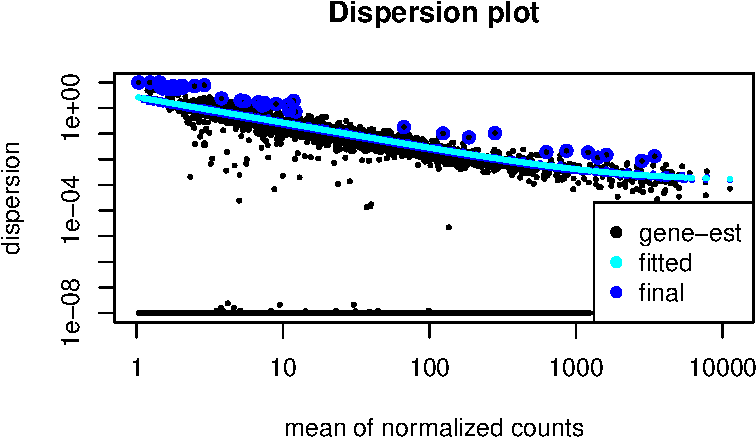
\includegraphics{intro-STAT-GroupProject_files/figure-pdf/unnamed-chunk-11-1.pdf}

}

\end{figure}

There's a trend where dispersion decreases as the mean of normalized
counts increases, which is typical in RNA-seq data due to biological
variability being more pronounced in genes with low expression levels.
The model (fitted line) captures the overall trend of the dispersion
estimates well, as indicated by the fitted points closely following the
line.

\begin{Shaded}
\begin{Highlighting}[]
\NormalTok{rld }\OtherTok{\textless{}{-}} \FunctionTok{rlogTransformation}\NormalTok{(dds) }\CommentTok{\#applies a regularized log transformation to the dds(DESeqDataSet)}

\CommentTok{\#Set colours for plotting}
\NormalTok{mycols }\OtherTok{\textless{}{-}} \FunctionTok{brewer.pal}\NormalTok{(}\DecValTok{8}\NormalTok{, }\StringTok{"Accent"}\NormalTok{)[}\DecValTok{1}\SpecialCharTok{:}\FunctionTok{length}\NormalTok{(}\FunctionTok{unique}\NormalTok{(condition))]}

\CommentTok{\# PCA}
\NormalTok{rld\_pca }\OtherTok{\textless{}{-}} \ControlFlowTok{function}\NormalTok{(rld, }\AttributeTok{intgroup =} \StringTok{"condition"}\NormalTok{, }\AttributeTok{ntop =} \DecValTok{500}\NormalTok{, }\AttributeTok{colors =} \ConstantTok{NULL}\NormalTok{, }\AttributeTok{legendpos =} \StringTok{"topright"}\NormalTok{, }\AttributeTok{main =} \StringTok{"PCA of regularized log foldchange of DE genes"}\NormalTok{, }\AttributeTok{textcx =} \DecValTok{1}\NormalTok{, ...) \{}
  
\NormalTok{  rv }\OtherTok{\textless{}{-}} \FunctionTok{rowVars}\NormalTok{(}\FunctionTok{assay}\NormalTok{(rld))}
\NormalTok{  select }\OtherTok{\textless{}{-}} \FunctionTok{order}\NormalTok{(rv, }\AttributeTok{decreasing =} \ConstantTok{TRUE}\NormalTok{)[}\FunctionTok{seq\_len}\NormalTok{(}\FunctionTok{min}\NormalTok{(ntop, }\FunctionTok{length}\NormalTok{(rv)))]}
\NormalTok{  pca }\OtherTok{\textless{}{-}} \FunctionTok{prcomp}\NormalTok{(}\FunctionTok{t}\NormalTok{(}\FunctionTok{assay}\NormalTok{(rld)[select, ]))}
\NormalTok{  fac }\OtherTok{\textless{}{-}} \FunctionTok{factor}\NormalTok{(}\FunctionTok{apply}\NormalTok{(}\FunctionTok{as.data.frame}\NormalTok{(}\FunctionTok{colData}\NormalTok{(rld)[, intgroup, }\AttributeTok{drop =} \ConstantTok{FALSE}\NormalTok{]), }\DecValTok{1}\NormalTok{, paste, }\AttributeTok{collapse =} \StringTok{" : "}\NormalTok{))}
  
\NormalTok{  pc1var }\OtherTok{\textless{}{-}} \FunctionTok{round}\NormalTok{(}\FunctionTok{summary}\NormalTok{(pca)}\SpecialCharTok{$}\NormalTok{importance[}\DecValTok{2}\NormalTok{, }\DecValTok{1}\NormalTok{] }\SpecialCharTok{*} \DecValTok{100}\NormalTok{, }\AttributeTok{digits =} \DecValTok{1}\NormalTok{)}
\NormalTok{  pc2var }\OtherTok{\textless{}{-}} \FunctionTok{round}\NormalTok{(}\FunctionTok{summary}\NormalTok{(pca)}\SpecialCharTok{$}\NormalTok{importance[}\DecValTok{2}\NormalTok{, }\DecValTok{2}\NormalTok{] }\SpecialCharTok{*} \DecValTok{100}\NormalTok{, }\AttributeTok{digits =} \DecValTok{1}\NormalTok{)}
\NormalTok{  pc1lab }\OtherTok{\textless{}{-}} \FunctionTok{paste0}\NormalTok{(}\StringTok{"PC1: "}\NormalTok{, }\FunctionTok{as.character}\NormalTok{(pc1var), }\StringTok{"\% variance"}\NormalTok{)}
\NormalTok{  pc2lab }\OtherTok{\textless{}{-}} \FunctionTok{paste0}\NormalTok{(}\StringTok{"PC2: "}\NormalTok{, }\FunctionTok{as.character}\NormalTok{(pc2var), }\StringTok{"\% variance"}\NormalTok{)}
  
  
  \FunctionTok{plot}\NormalTok{(PC2 }\SpecialCharTok{\textasciitilde{}}\NormalTok{ PC1, }\AttributeTok{data =} \FunctionTok{as.data.frame}\NormalTok{(pca}\SpecialCharTok{$}\NormalTok{x), }\AttributeTok{bg =}\NormalTok{ colors[fac], }\AttributeTok{pch =} \DecValTok{21}\NormalTok{, }\AttributeTok{xlab =}\NormalTok{ pc1lab, }\AttributeTok{ylab =}\NormalTok{ pc2lab, }\AttributeTok{main =}\NormalTok{ main, ...)}
  
  \FunctionTok{with}\NormalTok{(}\FunctionTok{as.data.frame}\NormalTok{(pca}\SpecialCharTok{$}\NormalTok{x), }\FunctionTok{textxy}\NormalTok{(PC1, PC2, }\AttributeTok{labs =} \FunctionTok{rownames}\NormalTok{(pca}\SpecialCharTok{$}\NormalTok{x), }\AttributeTok{cex =}\NormalTok{ textcx)) }
  \FunctionTok{legend}\NormalTok{(legendpos, }\AttributeTok{legend =} \FunctionTok{levels}\NormalTok{(fac), }\AttributeTok{col =}\NormalTok{ colors, }\AttributeTok{pch =} \DecValTok{20}\NormalTok{)}
\NormalTok{\}}

\FunctionTok{rld\_pca}\NormalTok{(rld, }\AttributeTok{colors =}\NormalTok{ mycols, }\AttributeTok{intgroup =} \StringTok{"condition"}\NormalTok{, }\AttributeTok{xlim =} \FunctionTok{c}\NormalTok{(}\SpecialCharTok{{-}}\DecValTok{15}\NormalTok{, }\DecValTok{20}\NormalTok{), }\AttributeTok{ylim =} \FunctionTok{c}\NormalTok{(}\SpecialCharTok{{-}}\DecValTok{10}\NormalTok{, }\DecValTok{10}\NormalTok{))}
\end{Highlighting}
\end{Shaded}

\begin{figure}[H]

{\centering 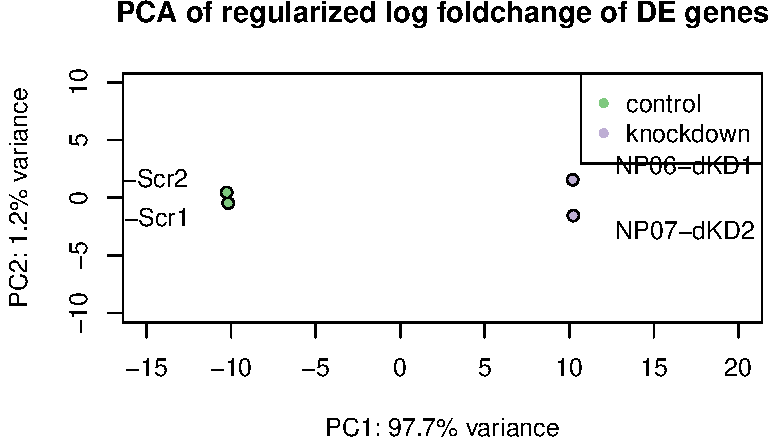
\includegraphics{intro-STAT-GroupProject_files/figure-pdf/unnamed-chunk-12-1.pdf}

}

\end{figure}

PCA further confirms there is little variability between biological
replicates but high variability between gene expression of control and
knockdown, indicating that the DRS long reads are capturing the
variability of the NMD knockdown at a gene expression level.

\begin{Shaded}
\begin{Highlighting}[]
\CommentTok{\# MA Plot}
\NormalTok{maplot }\OtherTok{\textless{}{-}} \ControlFlowTok{function}\NormalTok{ (res, }\AttributeTok{thresh =} \FloatTok{0.05}\NormalTok{, }\AttributeTok{labelsig =} \ConstantTok{FALSE}\NormalTok{, }\AttributeTok{textcx =} \DecValTok{1}\NormalTok{, ...) \{}
  \FunctionTok{with}\NormalTok{(res, }\FunctionTok{plot}\NormalTok{(baseMean, log2FoldChange, }\AttributeTok{pch =} \DecValTok{20}\NormalTok{, }\AttributeTok{cex =} \FloatTok{0.5}\NormalTok{, }\AttributeTok{log =} \StringTok{"x"}\NormalTok{, ...))}
  \FunctionTok{with}\NormalTok{(}\FunctionTok{subset}\NormalTok{(res, padj }\SpecialCharTok{\textless{}}\NormalTok{ thresh), }\FunctionTok{points}\NormalTok{(baseMean, log2FoldChange, }\AttributeTok{col =} \StringTok{"blue"}\NormalTok{, }\AttributeTok{pch =} \DecValTok{20}\NormalTok{, }\AttributeTok{cex =} \DecValTok{1}\NormalTok{))}
  \ControlFlowTok{if}\NormalTok{ (labelsig) \{}
    \FunctionTok{require}\NormalTok{(calibrate)}
    \FunctionTok{with}\NormalTok{(}\FunctionTok{subset}\NormalTok{(res, padj }\SpecialCharTok{\textless{}}\NormalTok{ thresh), }\FunctionTok{textxy}\NormalTok{(baseMean, log2FoldChange, }\AttributeTok{labs =}\NormalTok{ Gene, }\AttributeTok{cex =}\NormalTok{ textcx, }\AttributeTok{col =} \DecValTok{2}\NormalTok{))}
\NormalTok{  \}}
\NormalTok{\}}

\CommentTok{\# Volcano Plot}
\NormalTok{volcanoplot }\OtherTok{\textless{}{-}} \ControlFlowTok{function}\NormalTok{ (res, }\AttributeTok{lfcthresh =} \DecValTok{2}\NormalTok{, }\AttributeTok{sigthresh =} \FloatTok{0.05}\NormalTok{, }\AttributeTok{xlab =} \StringTok{"log2(Fold Change)"}\NormalTok{, }\AttributeTok{legendpos =} \StringTok{"topright"}\NormalTok{, }\AttributeTok{labelsig =} \ConstantTok{FALSE}\NormalTok{, }\AttributeTok{textcx =} \FloatTok{1.5}\NormalTok{, ...) \{}
  \FunctionTok{with}\NormalTok{(res, }\FunctionTok{plot}\NormalTok{(log2FoldChange, }\SpecialCharTok{{-}}\FunctionTok{log10}\NormalTok{(pvalue), }\AttributeTok{pch =} \DecValTok{20}\NormalTok{, }\AttributeTok{xlab =}\NormalTok{ xlab, }\AttributeTok{cex.axis =} \FloatTok{1.2}\NormalTok{, }\AttributeTok{cex.lab =} \FloatTok{1.2}\NormalTok{, ...))  }\CommentTok{\# Adjust cex.axis and cex.lab}
  \FunctionTok{with}\NormalTok{(}\FunctionTok{subset}\NormalTok{(res, padj }\SpecialCharTok{\textless{}}\NormalTok{ sigthresh), }\FunctionTok{points}\NormalTok{(log2FoldChange, }\SpecialCharTok{{-}}\FunctionTok{log10}\NormalTok{(pvalue), }\AttributeTok{pch =} \DecValTok{20}\NormalTok{, }\AttributeTok{col =} \StringTok{"blue"}\NormalTok{, ...))}
  \FunctionTok{with}\NormalTok{(}\FunctionTok{subset}\NormalTok{(res, }\FunctionTok{abs}\NormalTok{(log2FoldChange) }\SpecialCharTok{\textgreater{}}\NormalTok{ lfcthresh), }\FunctionTok{points}\NormalTok{(log2FoldChange, }\SpecialCharTok{{-}}\FunctionTok{log10}\NormalTok{(pvalue), }\AttributeTok{pch =} \DecValTok{20}\NormalTok{, }\AttributeTok{col =} \StringTok{"orange"}\NormalTok{, ...))}
  \FunctionTok{with}\NormalTok{(}\FunctionTok{subset}\NormalTok{(res, padj }\SpecialCharTok{\textless{}}\NormalTok{ sigthresh }\SpecialCharTok{\&} \FunctionTok{abs}\NormalTok{(log2FoldChange) }\SpecialCharTok{\textgreater{}}\NormalTok{ lfcthresh), }\FunctionTok{points}\NormalTok{(log2FoldChange, }\SpecialCharTok{{-}}\FunctionTok{log10}\NormalTok{(pvalue), }\AttributeTok{pch =} \DecValTok{20}\NormalTok{, }\AttributeTok{col =} \StringTok{"green"}\NormalTok{, ...))}
  \FunctionTok{legend}\NormalTok{(legendpos, }\AttributeTok{xjust =} \DecValTok{1}\NormalTok{, }\AttributeTok{yjust =} \DecValTok{1}\NormalTok{, }\AttributeTok{legend =} \FunctionTok{c}\NormalTok{(}\FunctionTok{paste}\NormalTok{(}\StringTok{"p{-}adj\textless{}"}\NormalTok{, sigthresh, }\AttributeTok{sep =} \StringTok{""}\NormalTok{), }\FunctionTok{paste}\NormalTok{(}\StringTok{"|log2(FC)|\textgreater{}"}\NormalTok{, lfcthresh, }\AttributeTok{sep =} \StringTok{""}\NormalTok{), }\StringTok{"both"}\NormalTok{), }\AttributeTok{cex =} \FloatTok{1.2}\NormalTok{, }\AttributeTok{pch =} \DecValTok{20}\NormalTok{, }\AttributeTok{col =} \FunctionTok{c}\NormalTok{(}\StringTok{"blue"}\NormalTok{, }\StringTok{"orange"}\NormalTok{, }\StringTok{"green"}\NormalTok{))  }\CommentTok{\# Adjust cex}
\NormalTok{\}}

\CommentTok{\# Set up the layout}
\FunctionTok{par}\NormalTok{(}\AttributeTok{mfrow =} \FunctionTok{c}\NormalTok{(}\DecValTok{1}\NormalTok{, }\DecValTok{2}\NormalTok{), }\AttributeTok{mar =} \FunctionTok{c}\NormalTok{(}\DecValTok{5}\NormalTok{, }\DecValTok{4}\NormalTok{, }\DecValTok{4}\NormalTok{, }\DecValTok{2}\NormalTok{) }\SpecialCharTok{+} \FloatTok{0.1}\NormalTok{)}

\CommentTok{\# Plot MA Plot}
\FunctionTok{maplot}\NormalTok{(resdata, }\AttributeTok{main =} \StringTok{"MA Plot"}\NormalTok{)}

\CommentTok{\# Plot Volcano Plot}
\FunctionTok{volcanoplot}\NormalTok{(resdata, }\AttributeTok{lfcthresh =} \DecValTok{2}\NormalTok{, }\AttributeTok{sigthresh =} \FloatTok{0.05}\NormalTok{, }\AttributeTok{xlim =} \FunctionTok{c}\NormalTok{(}\SpecialCharTok{{-}}\DecValTok{6}\NormalTok{, }\DecValTok{6}\NormalTok{), }\AttributeTok{ylim =} \FunctionTok{c}\NormalTok{(}\DecValTok{0}\NormalTok{, }\DecValTok{33}\NormalTok{), }\AttributeTok{legendpos =} \StringTok{"topright"}\NormalTok{, }\AttributeTok{main=}\StringTok{"Volcano plot"}\NormalTok{)}
\end{Highlighting}
\end{Shaded}

\begin{figure}[H]

{\centering 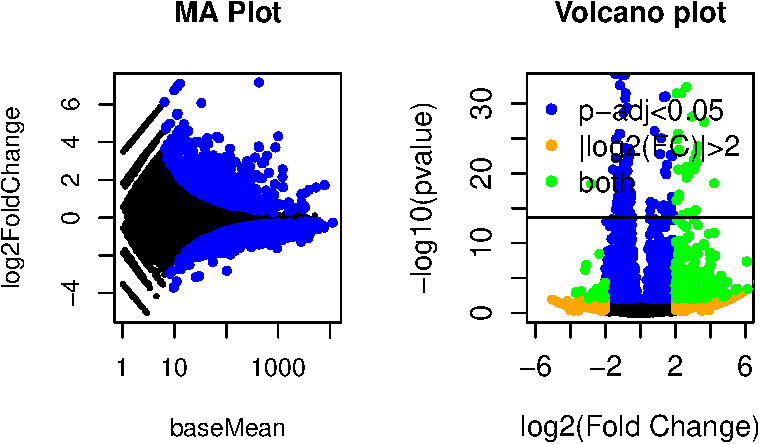
\includegraphics{intro-STAT-GroupProject_files/figure-pdf/unnamed-chunk-13-1.pdf}

}

\end{figure}

\begin{Shaded}
\begin{Highlighting}[]
\CommentTok{\# Reset the par settings to default after plotting}
\FunctionTok{par}\NormalTok{(}\AttributeTok{mfrow =} \FunctionTok{c}\NormalTok{(}\DecValTok{1}\NormalTok{, }\DecValTok{1}\NormalTok{), }\AttributeTok{mar =} \FunctionTok{c}\NormalTok{(}\DecValTok{5}\NormalTok{, }\DecValTok{4}\NormalTok{, }\DecValTok{4}\NormalTok{, }\DecValTok{2}\NormalTok{) }\SpecialCharTok{+} \FloatTok{0.1}\NormalTok{)}
\end{Highlighting}
\end{Shaded}

\hypertarget{differential-transcript-usage}{%
\section{Differential Transcript
Usage}\label{differential-transcript-usage}}

To asses w

\begin{Shaded}
\begin{Highlighting}[]
\NormalTok{sampleID }\OtherTok{=} \FunctionTok{c}\NormalTok{(}\StringTok{"tpm\_np05"}\NormalTok{,}\StringTok{"tpm\_np06"}\NormalTok{,}\StringTok{"tpm\_np07"}\NormalTok{,}\StringTok{"tpm\_np08"}\NormalTok{)}
\NormalTok{myDesign }\OtherTok{=} \FunctionTok{data.frame}\NormalTok{(}\AttributeTok{sampleID=}\NormalTok{ sampleID, }\AttributeTok{condition =}\NormalTok{ condition)}
\NormalTok{tpm\_transcriptome}\SpecialCharTok{$}\NormalTok{isoform\_id }\OtherTok{\textless{}{-}} \FunctionTok{rownames}\NormalTok{(tpm\_transcriptome)}

\NormalTok{aSwitchList }\OtherTok{\textless{}{-}} \FunctionTok{importRdata}\NormalTok{(}
  \AttributeTok{isoformCountMatrix   =}\NormalTok{ tpm\_transcriptome,}
  \AttributeTok{isoformRepExpression =}\NormalTok{ tpm\_transcriptome,}
  \AttributeTok{designMatrix         =}\NormalTok{ myDesign,}
  \AttributeTok{isoformExonAnnoation =} \StringTok{"files/Homo\_sapiens.GRCh38.110.chr\_patch\_hapl\_scaff.gtf"}\NormalTok{,}
  \AttributeTok{isoformNtFasta       =} \StringTok{"files/transcriptome\_reference.fa"}\NormalTok{,}
  \AttributeTok{showProgress =} \ConstantTok{FALSE}
\NormalTok{)}

\NormalTok{SwitchListFiltered }\OtherTok{\textless{}{-}} \FunctionTok{preFilter}\NormalTok{(}
  \AttributeTok{switchAnalyzeRlist =}\NormalTok{ aSwitchList,}
  \AttributeTok{geneExpressionCutoff =} \DecValTok{5}\NormalTok{,}
  \AttributeTok{isoformExpressionCutoff =} \DecValTok{5}\NormalTok{,}
  \AttributeTok{removeSingleIsoformGenes =} \ConstantTok{TRUE}\NormalTok{)}

\NormalTok{SwitchListAnalyzed }\OtherTok{\textless{}{-}} \FunctionTok{isoformSwitchTestDEXSeq}\NormalTok{(}
  \AttributeTok{switchAnalyzeRlist =}\NormalTok{ SwitchListFiltered,}
  \AttributeTok{reduceToSwitchingGenes=}\ConstantTok{TRUE}\NormalTok{,}
  \AttributeTok{reduceFurtherToGenesWithConsequencePotential =} \ConstantTok{FALSE}\NormalTok{,}
  \AttributeTok{alpha =} \FloatTok{0.05}\NormalTok{,}
  \AttributeTok{dIFcutoff =} \FloatTok{0.1}\NormalTok{,}
  \AttributeTok{onlySigIsoforms =} \ConstantTok{FALSE}
\NormalTok{)}

\FunctionTok{extractSwitchSummary}\NormalTok{(SwitchListAnalyzed)}
\NormalTok{summary\_isoforms }\OtherTok{\textless{}{-}}\NormalTok{ SwitchListAnalyzed}\SpecialCharTok{$}\NormalTok{isoformFeatures}
\FunctionTok{write.csv}\NormalTok{(summary\_isoforms[(summary\_isoforms}\SpecialCharTok{$}\NormalTok{iso\_biotype }\SpecialCharTok{==} \StringTok{"nonsense\_mediated\_decay"}\NormalTok{),], }\StringTok{"NMD\_isoformfeatures.tr.csv"}\NormalTok{)}
\end{Highlighting}
\end{Shaded}

\begin{Shaded}
\begin{Highlighting}[]
\NormalTok{new\_nmd }\OtherTok{=} \FunctionTok{read.csv}\NormalTok{(}\AttributeTok{file =} \StringTok{\textquotesingle{}NMD\_exons\_to\_long\_reads\_transcriptome\_mapping.csv\textquotesingle{}}\NormalTok{, }\AttributeTok{sep =} \StringTok{\textquotesingle{},\textquotesingle{}}\NormalTok{, }\AttributeTok{header =} \ConstantTok{TRUE}\NormalTok{)}
\end{Highlighting}
\end{Shaded}

\hypertarget{splicing-analysis}{%
\subsection{Splicing Analysis}\label{splicing-analysis}}

Furthermore, we use SplAdder (\textbf{kahles2016spladder?}) to perform a
differential splicing analysis similar to (Karousis et al. 2021).
SplAdder first generates a splicing graph based on the RNA sequencing
data and extracts alternative splicing events (compared to the reference
genome). The detected splicing events correspond to single or multiple
skipped exons, intron retentions, alternative 3' or 5' splicing, and
mutually exclusive exons. In a second step, it runs a differential test
in order to find events that occur with a significantly different
frequency in the knockdown samples compared to wildtype.

\begin{Shaded}
\begin{Highlighting}[]
\BuiltInTok{echo} \StringTok{"build splicing graph"}

\ExtensionTok{python} \AttributeTok{{-}m}\NormalTok{ spladder.spladder build }\AttributeTok{{-}{-}annotation} \VariableTok{$annotationFile} \DataTypeTok{\textbackslash{}}
                                  \AttributeTok{{-}{-}bams} \VariableTok{$wt1}\NormalTok{,}\VariableTok{$wt2}\NormalTok{,}\VariableTok{$kd1}\NormalTok{,}\VariableTok{$kd2} \DataTypeTok{\textbackslash{}}
                                  \AttributeTok{{-}{-}outdir} \VariableTok{$outFolder}

\BuiltInTok{echo} \StringTok{"run differential splicing analyis"}

\ExtensionTok{python} \AttributeTok{{-}m}\NormalTok{ spladder.spladder test }\DataTypeTok{\textbackslash{}}
              \AttributeTok{{-}{-}conditionA} \VariableTok{$wt1}\NormalTok{,}\VariableTok{$wt2} \DataTypeTok{\textbackslash{}}
              \AttributeTok{{-}{-}conditionB} \VariableTok{$kd1}\NormalTok{,}\VariableTok{$kd2} \DataTypeTok{\textbackslash{}}
              \AttributeTok{{-}{-}parallel}\NormalTok{ 24 }\DataTypeTok{\textbackslash{}}
              \AttributeTok{{-}{-}outdir} \VariableTok{$outFolder}
\end{Highlighting}
\end{Shaded}

\begin{Shaded}
\begin{Highlighting}[]
\CommentTok{\# we load all by SplAdder detected events and merge them into one table}

\NormalTok{alt\_3prime }\OtherTok{\textless{}{-}} \FunctionTok{as.data.frame}\NormalTok{(}\FunctionTok{read.table}\NormalTok{(}\StringTok{"splicing/test\_results\_C3\_alt\_3prime.tsv"}\NormalTok{, }\AttributeTok{sep =} \StringTok{"}\SpecialCharTok{\textbackslash{}t}\StringTok{"}\NormalTok{, }\AttributeTok{header =} \ConstantTok{TRUE}\NormalTok{))}
\NormalTok{alt\_5prime }\OtherTok{\textless{}{-}} \FunctionTok{as.data.frame}\NormalTok{(}\FunctionTok{read.table}\NormalTok{(}\StringTok{"splicing/test\_results\_C3\_alt\_5prime.tsv"}\NormalTok{, }\AttributeTok{sep =} \StringTok{"}\SpecialCharTok{\textbackslash{}t}\StringTok{"}\NormalTok{, }\AttributeTok{header =} \ConstantTok{TRUE}\NormalTok{))}
\NormalTok{exon\_skip }\OtherTok{\textless{}{-}} \FunctionTok{as.data.frame}\NormalTok{(}\FunctionTok{read.table}\NormalTok{(}\StringTok{"splicing/test\_results\_C3\_exon\_skip.tsv"}\NormalTok{, }\AttributeTok{sep =} \StringTok{"}\SpecialCharTok{\textbackslash{}t}\StringTok{"}\NormalTok{, }\AttributeTok{header =} \ConstantTok{TRUE}\NormalTok{))}
\NormalTok{intron\_retention }\OtherTok{\textless{}{-}} \FunctionTok{as.data.frame}\NormalTok{(}\FunctionTok{read.table}\NormalTok{(}\StringTok{"splicing/test\_results\_C3\_intron\_retention.tsv"}\NormalTok{, }\AttributeTok{sep =} \StringTok{"}\SpecialCharTok{\textbackslash{}t}\StringTok{"}\NormalTok{, }\AttributeTok{header =} \ConstantTok{TRUE}\NormalTok{))}
\NormalTok{mult\_exon\_skip }\OtherTok{\textless{}{-}} \FunctionTok{as.data.frame}\NormalTok{(}\FunctionTok{read.table}\NormalTok{(}\StringTok{"splicing/test\_results\_C3\_mult\_exon\_skip.tsv"}\NormalTok{, }\AttributeTok{sep =} \StringTok{"}\SpecialCharTok{\textbackslash{}t}\StringTok{"}\NormalTok{, }\AttributeTok{header =} \ConstantTok{TRUE}\NormalTok{))}
\NormalTok{mutex\_exons }\OtherTok{\textless{}{-}} \FunctionTok{as.data.frame}\NormalTok{(}\FunctionTok{read.table}\NormalTok{(}\StringTok{"splicing/test\_results\_C3\_mutex\_exons.tsv"}\NormalTok{, }\AttributeTok{sep =} \StringTok{"}\SpecialCharTok{\textbackslash{}t}\StringTok{"}\NormalTok{, }\AttributeTok{header =} \ConstantTok{TRUE}\NormalTok{))}


\NormalTok{alt\_3prime }\OtherTok{\textless{}{-}} \FunctionTok{transform}\NormalTok{(alt\_3prime, }\AttributeTok{Type=}\StringTok{"alt\_3prime"}\NormalTok{)}
\NormalTok{alt\_5prime }\OtherTok{\textless{}{-}} \FunctionTok{transform}\NormalTok{(alt\_5prime, }\AttributeTok{Type=}\StringTok{"alt\_5prime"}\NormalTok{)}
\NormalTok{exon\_skip }\OtherTok{\textless{}{-}} \FunctionTok{transform}\NormalTok{(exon\_skip, }\AttributeTok{Type=}\StringTok{"exon\_skip"}\NormalTok{)}
\NormalTok{intron\_retention }\OtherTok{\textless{}{-}} \FunctionTok{transform}\NormalTok{(intron\_retention, }\AttributeTok{Type=}\StringTok{"intron\_retention"}\NormalTok{)}
\NormalTok{mult\_exon\_skip }\OtherTok{\textless{}{-}} \FunctionTok{transform}\NormalTok{(mult\_exon\_skip, }\AttributeTok{Type=}\StringTok{"mult\_exon\_skip"}\NormalTok{)}
\NormalTok{mutex\_exons }\OtherTok{\textless{}{-}} \FunctionTok{transform}\NormalTok{(mutex\_exons, }\AttributeTok{Type=}\StringTok{"mutex\_exons"}\NormalTok{)}

\NormalTok{splicing\_events }\OtherTok{\textless{}{-}} \FunctionTok{Reduce}\NormalTok{(}\ControlFlowTok{function}\NormalTok{(x, y) }\FunctionTok{merge}\NormalTok{(x, y, }\AttributeTok{all=}\ConstantTok{TRUE}\NormalTok{), }\FunctionTok{list}\NormalTok{(}
\NormalTok{  alt\_3prime,}
\NormalTok{  alt\_5prime,}
\NormalTok{  exon\_skip,}
\NormalTok{  intron\_retention,}
\NormalTok{  mult\_exon\_skip,}
\NormalTok{  mutex\_exons}
\NormalTok{))}

\CommentTok{\# filter only significant events}
\NormalTok{splicing\_events }\OtherTok{\textless{}{-}}\NormalTok{ splicing\_events[splicing\_events}\SpecialCharTok{$}\NormalTok{p\_val\_adj }\SpecialCharTok{\textless{}} \FloatTok{0.05}\NormalTok{,]}
\end{Highlighting}
\end{Shaded}

We first plot the number of events per event type and the number of
unique genes per event type:

\begin{Shaded}
\begin{Highlighting}[]
\NormalTok{event\_counts\_per\_event\_type }\OtherTok{\textless{}{-}}\NormalTok{ splicing\_events }\SpecialCharTok{\%\textgreater{}\%}
  \FunctionTok{group\_by}\NormalTok{(Type) }\SpecialCharTok{\%\textgreater{}\%}
  \FunctionTok{summarise}\NormalTok{(}\AttributeTok{UniqueCount =} \FunctionTok{n\_distinct}\NormalTok{(event\_id))}

\NormalTok{gene\_counts\_per\_event\_type }\OtherTok{\textless{}{-}}\NormalTok{ splicing\_events }\SpecialCharTok{\%\textgreater{}\%}
  \FunctionTok{group\_by}\NormalTok{(Type) }\SpecialCharTok{\%\textgreater{}\%}
  \FunctionTok{summarise}\NormalTok{(}\AttributeTok{UniqueCount =} \FunctionTok{n\_distinct}\NormalTok{(gene\_id))}

\FunctionTok{ggplot}\NormalTok{(event\_counts\_per\_event\_type, }\FunctionTok{aes}\NormalTok{(}\AttributeTok{x =}\NormalTok{ Type, }\AttributeTok{y =}\NormalTok{ UniqueCount)) }\SpecialCharTok{+}
  \FunctionTok{geom\_bar}\NormalTok{(}\AttributeTok{stat =} \StringTok{"identity"}\NormalTok{) }\SpecialCharTok{+}
  \FunctionTok{ylim}\NormalTok{(}\DecValTok{0}\NormalTok{, }\DecValTok{250}\NormalTok{) }\SpecialCharTok{+} 
  \FunctionTok{labs}\NormalTok{(}\AttributeTok{x =} \StringTok{"Splicing Event Type"}\NormalTok{,}
       \AttributeTok{y =} \StringTok{"Number Events"}\NormalTok{) }\SpecialCharTok{+}
  \FunctionTok{theme\_minimal}\NormalTok{() }\SpecialCharTok{+}
  \FunctionTok{scale\_x\_discrete}\NormalTok{(}\AttributeTok{guide =} \FunctionTok{guide\_axis}\NormalTok{(}\AttributeTok{n.dodge =} \DecValTok{2}\NormalTok{)) }\SpecialCharTok{+}
  \FunctionTok{ggplot}\NormalTok{(gene\_counts\_per\_event\_type, }\FunctionTok{aes}\NormalTok{(}\AttributeTok{x =}\NormalTok{ Type, }\AttributeTok{y =}\NormalTok{ UniqueCount)) }\SpecialCharTok{+}
  \FunctionTok{ylim}\NormalTok{(}\DecValTok{0}\NormalTok{, }\DecValTok{250}\NormalTok{) }\SpecialCharTok{+} 
  \FunctionTok{geom\_bar}\NormalTok{(}\AttributeTok{stat =} \StringTok{"identity"}\NormalTok{) }\SpecialCharTok{+}
  \FunctionTok{labs}\NormalTok{(}\AttributeTok{x =} \StringTok{"Splicing Event Type"}\NormalTok{,}
       \AttributeTok{y =} \StringTok{"Number Genes With Events"}\NormalTok{) }\SpecialCharTok{+}
  \FunctionTok{scale\_x\_discrete}\NormalTok{(}\AttributeTok{guide =} \FunctionTok{guide\_axis}\NormalTok{(}\AttributeTok{n.dodge =} \DecValTok{2}\NormalTok{)) }\SpecialCharTok{+}
  \FunctionTok{theme\_minimal}\NormalTok{()}
\end{Highlighting}
\end{Shaded}

Furthermore, we can use SplAdder to confirm different splicing behavior
previously reported in literature. One example is the
apoptosis-modulating Bcl-2-associated athanogene-1 (BAG-1). (Karousis et
al. 2021) reported that a BAG1 isoform with an included alternative exon
is stabilized upon NMD inhibition. This effect can also be observed in
our data set:

\begin{Shaded}
\begin{Highlighting}[]
\BuiltInTok{echo} \StringTok{"run differential splicing analyis"}

\ExtensionTok{python} \AttributeTok{{-}m}\NormalTok{ spladder.spladder viz }\DataTypeTok{\textbackslash{}}
              \AttributeTok{{-}{-}range}\NormalTok{ gene ENSG00000107262 }\DataTypeTok{\textbackslash{}}
              \AttributeTok{{-}{-}track}\NormalTok{ coverage wildtype:}\VariableTok{$wt1}\NormalTok{,}\VariableTok{$wt2}\NormalTok{ knockdown:}\VariableTok{$kd1}\NormalTok{,}\VariableTok{$kd2} \DataTypeTok{\textbackslash{}}
              \AttributeTok{{-}{-}track}\NormalTok{ event exon\_skip }\DataTypeTok{\textbackslash{}}
              \AttributeTok{{-}O}\NormalTok{ plot }\AttributeTok{{-}{-}format}\NormalTok{ png }\DataTypeTok{\textbackslash{}}
              \AttributeTok{{-}{-}outdir} \VariableTok{$outFolder}
\end{Highlighting}
\end{Shaded}

\begin{figure}

{\centering 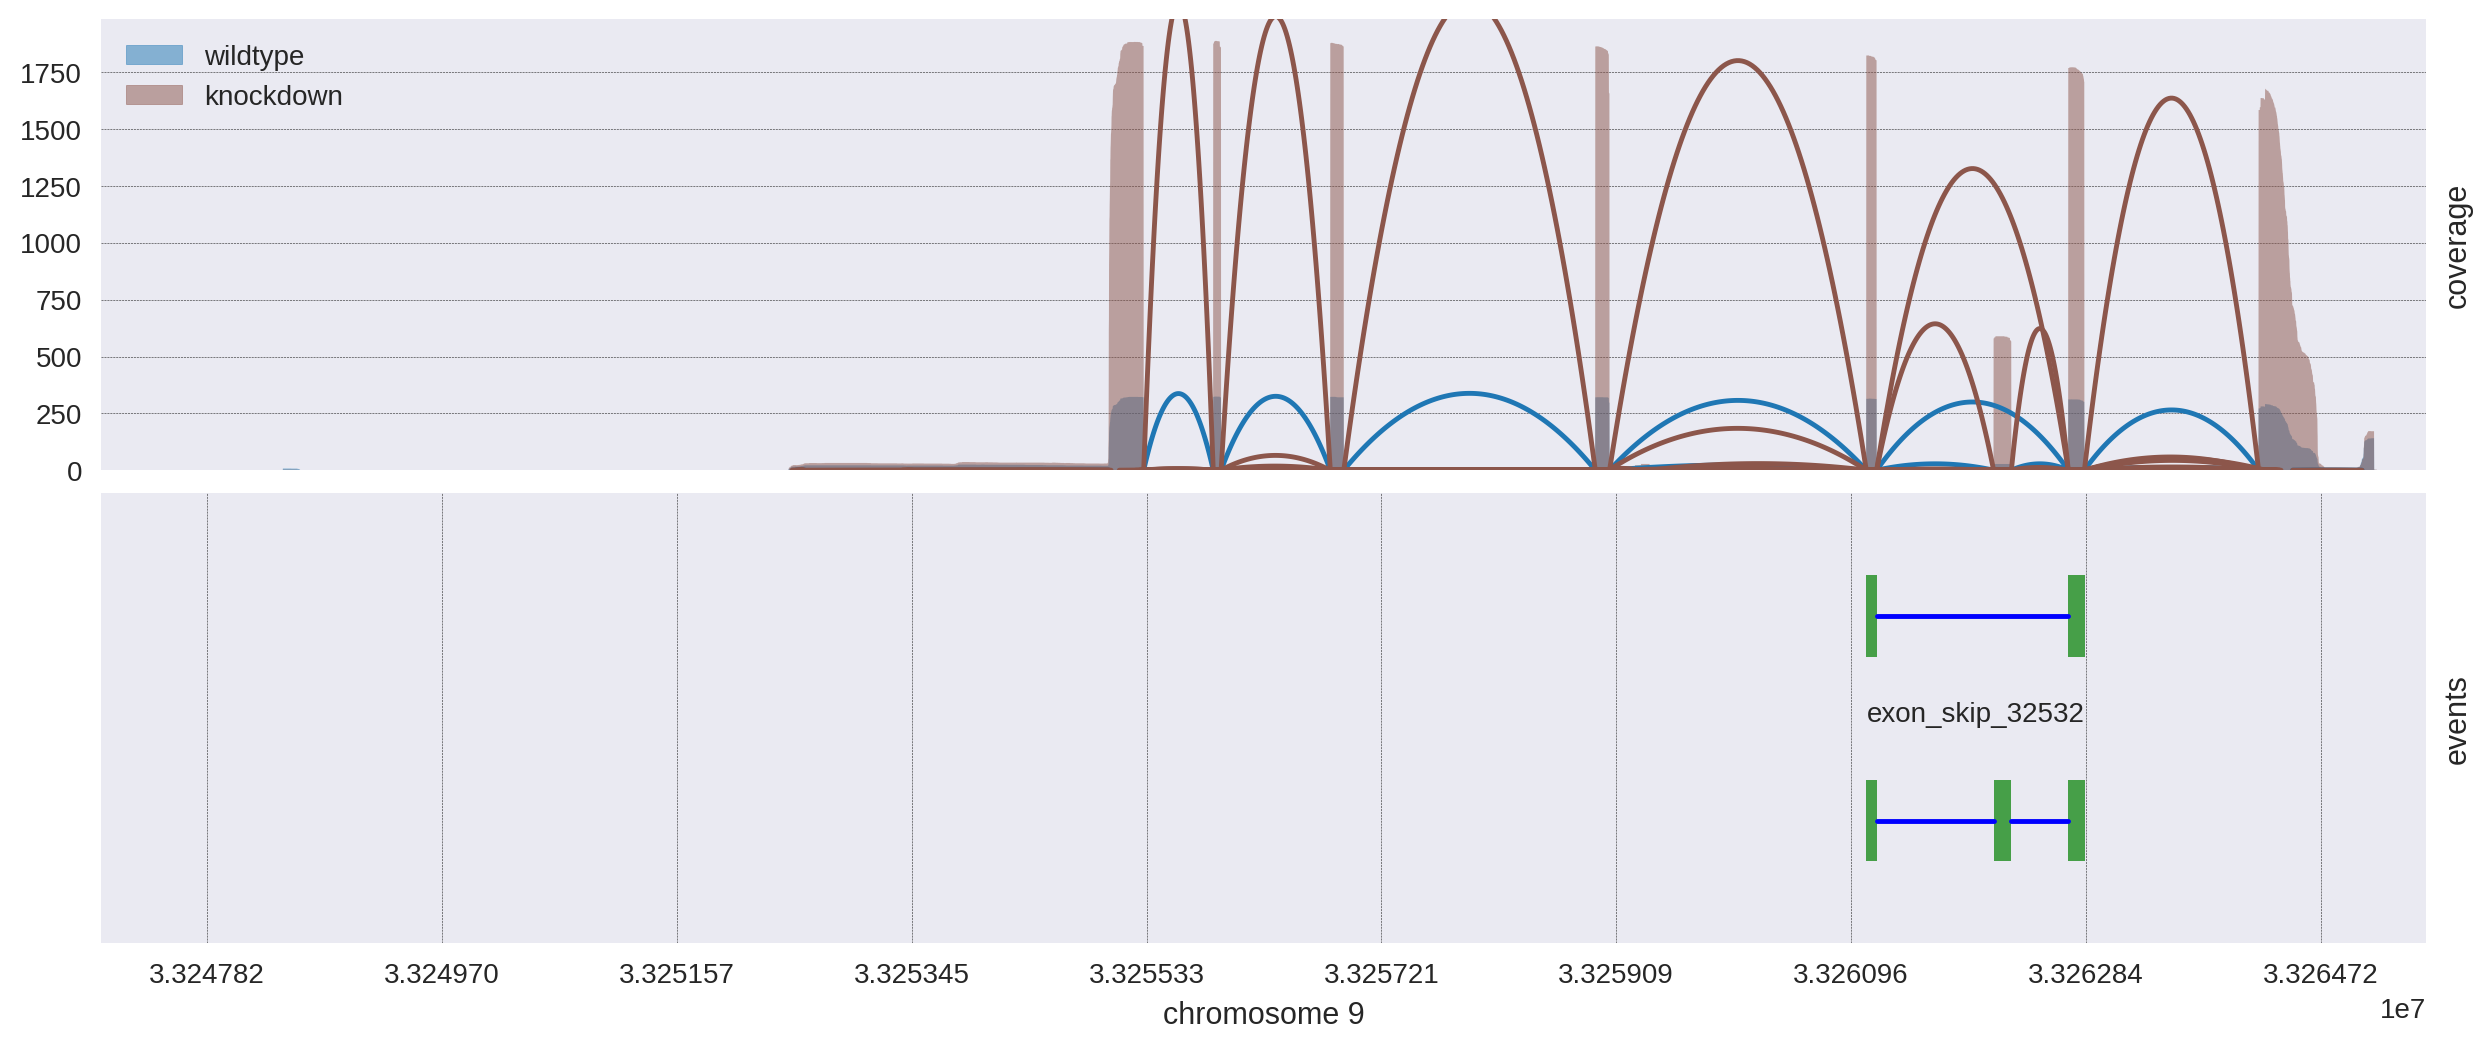
\includegraphics{splicing/plot.png}

}

\caption{SplAdder Analysis of the BAG-1 Gene. One can observe that an
alternative isoform is predominant in the knockdown sample, an
observation that is in line with previous literature.}

\end{figure}

\hypertarget{discovery-of-new-isoforms}{%
\subsection{Discovery of New Isoforms}\label{discovery-of-new-isoforms}}

We use FLAIR (\textbf{flair?}) to detect new isoforms in the sequences
of the knockdown samples when compared to the reference transcriptome.

\begin{Shaded}
\begin{Highlighting}[]
\ExtensionTok{python} \AttributeTok{{-}m}\NormalTok{ flair.flair correct }\DataTypeTok{\textbackslash{}}
\NormalTok{{-}{-}gtf }\VariableTok{$annotationFile} \DataTypeTok{\textbackslash{}}
\NormalTok{{-}{-}genome }\VariableTok{$referenceFile} \DataTypeTok{\textbackslash{}}
\NormalTok{{-}{-}query }\VariableTok{$experimentFolder}\NormalTok{/alignments/primary{-}genomic{-}aln.bed12 }\DataTypeTok{\textbackslash{}}
\NormalTok{{-}{-}output }\VariableTok{$experimentFolder}\NormalTok{/flair/correct}

\ExtensionTok{python} \AttributeTok{{-}m}\NormalTok{ flair.flair collapse }\DataTypeTok{\textbackslash{}}
\NormalTok{{-}{-}gtf }\VariableTok{$annotationFile} \DataTypeTok{\textbackslash{}}
\NormalTok{{-}{-}reads }\VariableTok{$rawReads} \DataTypeTok{\textbackslash{}}
\NormalTok{{-}{-}genome }\VariableTok{$referenceFile} \DataTypeTok{\textbackslash{}}
\NormalTok{{-}{-}query }\VariableTok{$experimentFolder}\NormalTok{/flair/correct\_all\_corrected.bed }\DataTypeTok{\textbackslash{}}
\NormalTok{{-}{-}trust\_ends }\DataTypeTok{\textbackslash{}}
\NormalTok{{-}{-}stringent }\DataTypeTok{\textbackslash{}}
\NormalTok{{-}{-}threads 16 }\DataTypeTok{\textbackslash{}}
\NormalTok{{-}{-}output }\VariableTok{$experimentFolder}\NormalTok{/flair/collapse}

\ExtensionTok{/cluster/home/ochsneto/gffcompare{-}0.12.6.Linux\_x86\_64/gffcompare} \AttributeTok{{-}r} \VariableTok{$annotationFile} \AttributeTok{{-}o} \VariableTok{$experimentFolder}\NormalTok{/flair/gffcompare }\AttributeTok{{-}V} \VariableTok{$experimentFolder}\NormalTok{/flair/collapse.isoforms.gtf}
\end{Highlighting}
\end{Shaded}

\hypertarget{references}{%
\subsubsection{References}\label{references}}

\hypertarget{refs}{}
\begin{CSLReferences}{1}{0}
\leavevmode\vadjust pre{\hypertarget{ref-aird2011analyzing}{}}%
Aird, Daniel, Michael G Ross, Wei-Sheng Chen, Maxwell Danielsson,
Timothy Fennell, Carsten Russ, David B Jaffe, Chad Nusbaum, and Andreas
Gnirke. 2011. {``Analyzing and Minimizing PCR Amplification Bias in
Illumina Sequencing Libraries.''} \emph{Genome Biology} 12 (2): 1--14.

\leavevmode\vadjust pre{\hypertarget{ref-gleeson2022accurate}{}}%
Gleeson, Josie, Adrien Leger, Yair DJ Prawer, Tracy A Lane, Paul J
Harrison, Wilfried Haerty, and Michael B Clark. 2022. {``Accurate
Expression Quantification from Nanopore Direct RNA Sequencing with
NanoCount.''} \emph{Nucleic Acids Research} 50 (4): e19--19.

\leavevmode\vadjust pre{\hypertarget{ref-karousis2021nanopore}{}}%
Karousis, Evangelos D, Foivos Gypas, Mihaela Zavolan, and Oliver
Mühlemann. 2021. {``Nanopore Sequencing Reveals Endogenous NMD-Targeted
Isoforms in Human Cells.''} \emph{Genome Biology} 22 (1): 1--23.

\leavevmode\vadjust pre{\hypertarget{ref-karousis2022broader}{}}%
Karousis, Evangelos D, and Oliver Mühlemann. 2022. {``The Broader Sense
of Nonsense.''} \emph{Trends in Biochemical Sciences}.

\leavevmode\vadjust pre{\hypertarget{ref-roundtree2017dynamic}{}}%
Roundtree, Ian A, Molly E Evans, Tao Pan, and Chuan He. 2017. {``Dynamic
RNA Modifications in Gene Expression Regulation.''} \emph{Cell} 169 (7):
1187--1200.

\leavevmode\vadjust pre{\hypertarget{ref-steijger2013assessment}{}}%
Steijger, Tamara, Josep F Abril, Pär G Engström, Felix Kokocinski, Tim J
Hubbard, Roderic Guigó, Jennifer Harrow, and Paul Bertone. 2013.
{``Assessment of Transcript Reconstruction Methods for RNA-Seq.''}
\emph{Nature Methods} 10 (12): 1177--84.

\end{CSLReferences}



\end{document}
